\documentclass[a4paper]{article}
\usepackage[utf8]{inputenc}
\usepackage[italian]{babel}
\usepackage[T1]{fontenc}
\usepackage{fancyhdr}
\usepackage{graphicx}
\usepackage{amssymb}
\usepackage{enumitem}
\usepackage{amsthm}
\usepackage[parfill]{parskip}
\usepackage{amsmath}
\usepackage[bookmarks=true]{hyperref}
\usepackage{mathtools}
\usepackage{gensymb} %contiene \degree
\usepackage{wasysym} %contiene gli altri comandi qui sotto
\let\leftmoon\relax
\let\rightmoon\relax
\let\fullmoon\relax
\let\newmoon\relax
\let\diameter\relax
\let\degree\relax
\usepackage{mathabx}\changenotsign %senza quest'ultimo comando viene | invece che /
\usepackage{dsfont}
\usepackage{tikz}
\usepackage{pgfplots}
\usepackage{bigints}
\usepackage[scr=boondox]{mathalfa}
\usepackage{centernot}
\usepackage{ifthen}
\usepackage{pdfpages}
\usepackage{xfrac}
\usepackage{nicefrac}
\usepackage{etaremune}
\usepackage{float}
\usepackage{chngcntr}
\usepackage{needspace}
\usepackage{imakeidx}
\usepackage{makecell}
\usepackage[it-IT]{datetime2}
\usepackage[makeroom]{cancel}
\usepackage{bm}
\usepackage{fontspec}

\usepackage[paperwidth=17cm, paperheight=24cm, twoside, left=2.5cm, right=2cm, top=2.5cm, bottom=3cm]{geometry}
% \usepackage{draftwatermark}
% \SetWatermarkText{\textsf{BOZZA}}
% \SetWatermarkScale{1}

\usetikzlibrary{patterns}
\counterwithin{figure}{section}
\renewcommand\arraystretch{1.3}

\pagestyle{fancy}
\fancyhf{}

\newtheoremstyle{break}% <name>
{3pt}% <Space above>
{3pt}% <Space below>
{\addtolength{\leftskip}{1.3em}}% <Body font>
{-1.13em}% <Indent amount>
{\bfseries}% <Theorem head font>
{}% <Punctuation after theorem head>
{\newline}% <Space after theorem head>
{}% <Theorem head spec (can be left empty, meaning `normal')>

\newtheoremstyle{breakb}% <name>
{3pt}% <Space above>
{3pt}% <Space below>
{\addtolength{\leftskip}{1.3em}}% <Body font>
{-1.13em}% <Indent amount>
{\bfseries}% <Theorem head font>
{}% <Punctuation after theorem head>
{\newline}% <Space after theorem head>
{\thmname{#1} \thmnumber{#2}\thmnote{ #3}}% <Theorem head spec (can be left empty, meaning `normal')>

\newtheoremstyle{breakit}% <name>
{3pt}% <Space above>
{3pt}% <Space below>
{}% <Body font>
{0em}% <Indent amount>
{}% <Theorem head font>
{.}% <Punctuation after theorem head>
{ }% <Space after theorem head>
{\textit{\thmname{#1}}\thmnote{: #3}}% <Theorem head spec (can be left empty, meaning `normal')>

\newtheoremstyle{breakitb}% <name>
{3pt}% <Space above>
{3pt}% <Space below>
{}% <Body font>
{0em}% <Indent amount>
{}% <Theorem head font>
{}% <Punctuation after theorem head>
{ }% <Space after theorem head>
{\textit{\thmname{#1}}\thmnote{ #3}}% <Theorem head spec (can be left empty, meaning `normal')>

\newtheoremstyle{bold}% <name>
{3pt}% <Space above>
{3pt}% <Space below>
{\addtolength{\leftskip}{1.3em}}% <Body font>
{-1.13em}% <Indent amount>
{\bfseries}% <Theorem head font>
{:}% <Punctuation after theorem head>
{.5em}% <Space after theorem head>
{}% <Theorem head spec (can be left empty, meaning `normal')>

\hypersetup{
     colorlinks = true,
     citecolor  = gray,
     urlcolor   = black
}

\newenvironment{firma}
  {\par\hfill\itshape
   \begin{tabular}{@{}r@{\hspace{2em}}}} % 2em from the right margin
  {\end{tabular}\par\medskip}

\fancypagestyle{inner}{%
  \fancyhf{}% Clear header/footer
  \fancyhead[OR]{\rightmark}
  \fancyhead[EL]{\leftmark}
  \fancyfoot[OR]{\thepage}
  \fancyfoot[EL]{\thepage}
  \renewcommand{\headrulewidth}{0.1pt}% Header rule of .4pt
}
\renewcommand{\sectionmark}[1]{\markboth{\thesection.~#1}{}}

\definecolor{battleshipgrey}{rgb}{0.52, 0.52, 0.51}
\fancypagestyle{foglio}{%
  \fancyhf{}% Clear header/footer
  \fancyfoot[R]{\raisebox{1.8em}{
  	{\footnotesize \color{battleshipgrey} \ttfamily Fubini$\otimes$Tonelli - Appunti di probabilità - fubinitonelli.it}
  }}
  \fancyfoot[L]{\raisebox{1.8em}{{\footnotesize \color{battleshipgrey} \ttfamily \thepage}}}
  \renewcommand{\headrulewidth}{0.0pt}
}

\fancypagestyle{plain}{%
  \fancyhf{}% Clear header/footer
  \fancyfoot[OR]{\thepage}
  \fancyfoot[EL]{\thepage}
  \renewcommand{\headrulewidth}{0.0pt}% Header rule of .4pt
}

\makeatletter
% case 1: theorem name--number ("ordinary") style
\patchcmd{\thmhead@plain}%
   {\thmnote{ {\the\thm@notefont(#3)}}}%  original form
   {\thmnote{:  #3}}%  new form
   {}{}
\let\thmhead\thmhead@plain

%\renewcommand{\qed}{\hfill \ensuremath{\Box}}

\theoremstyle{break}
\newtheorem{teo}{Teorema}[section]
\newtheorem{coro}[teo]{Corollario}
\newtheorem{defn}[teo]{Definizione}
\newtheorem{oss}[teo]{Osservazione}
\newtheorem{prop}[teo]{Proposizione}
\newtheorem{lemma}[teo]{Lemma}

\theoremstyle{breakb}
\newtheorem{teob}[teo]{Teorema}
\newtheorem{corob}[teo]{Corollario}
\newtheorem{propb}[teo]{Proposizione}
\newtheorem*{XxmpX}{Dimostrazione}
\newenvironment{dimo}    % this is the environment name for the input
  {\pushQED{\qed}\begin{XxmpX}}
   {\popQED\end{XxmpX}}

\theoremstyle{bold}
\newtheorem*{nb}{NB}

\theoremstyle{breakit}
\newtheorem*{ese}{Esempio}
\newtheorem*{eser}{Esercizio}
\newtheorem*{cese}{Controesempio}

\theoremstyle{breakitb}
\newtheorem*{eseb}{Esempio}
\newtheorem*{eserb}{Esercizio}
\newtheorem*{ceseb}{Controesempio}

\DeclarePairedDelimiter\abs{\lvert}{\rvert}
\DeclarePairedDelimiter\norm{\lVert}{\rVert}
\DeclarePairedDelimiter{\ceil}{\lceil}{\rceil}

\newcommand\sigmaeq{\stackrel{\mathclap{\normalfont\mbox{$\sigma$-add}}}{\quad=\quad}}
\newcommand\aceq{\stackrel{\mathclap{\normalfont\mbox{qc}}}{\;=\;}}
\newcommand{\indep}{\mathrel{\text{\scalebox{1.07}{$\perp\mkern-10mu\perp$}}}}
\newcommand{\padtwo}[1]{\ifnum #1 < 10 0\fi #1}

\newcommand{\lezione}[2]{}

\newcommand{\esercitazione}[2]{}

\newenvironment{dedication}
  {\clearpage           % we want a new page
   \thispagestyle{empty}% no header and footer
   \vspace*{\stretch{1}}% some space at the top
   \itshape             % the text is in italics
   \raggedleft          % flush to the right margin
  }
  {\par % end the paragraph
   \vspace{\stretch{2}} % space at bottom is three times that at the top
   \cleardoublepage     % finish off the page
  }

\newcommand*{\blankpage}{%

}

%cleardoublepage lascia le pagine bianche, con solo il numero
\makeatletter
\def\emptypage@emptypage{%
    \hbox{}%
    \thispagestyle{plain}   %% or any page style
    \blankpage%
    \newpage%
}%
\def\cleardoublepage{%
        \clearpage%
        \if@twoside%
            \ifodd\c@page%
                % do nothing
            \else%
                \emptypage@emptypage%
            \fi%
        \fi%
    }%
\makeatother

% SCORCIATOIE PERSONALIZZATE

%% Formattazione
\newcommand{\Fixvmode}{\leavevmode\vspace{-\baselineskip}}
\newcommand{\JPTh}[1]{\normalfont{(\textit{J-P Th #1})}}
\newcommand{\JPCoro}[1]{\normalfont{(\textit{J-P Coro #1})}}

%% Varie
\newcommand{\DimStar}{
  \textit{\framebox[2.5\width]{$\ast$} La dimostrazione sotto riportata fa parte del solo programma completo.}
}

\newcommand{\DimStarPar}{
  \textit{\framebox[2.5\width]{$\ast$!} Una parte della dimostrazione sotto riportata fa parte del solo programma completo.}
}
\newcommand{\DimStarInd}{
  \textit{\framebox[2.5\width]{$\ast$} Questa parte della dimostrazione fa parte del solo programma completo.}
}
\newcommand{\EsStar}{
  \textit{\framebox[2.5\width]{$\ast$} L'esempio sotto riportato fa parte del solo programma completo.}
}

\newcommand{\DoCo}[1][n]{(\Omega, \Ac, \PP) \to \ifthenelse{\equal{#1}{1}}{(\RR, \Bc)}{(\RR^{#1}, \Bc^{#1})}}
\newcommand{\Dom}{(\Omega, \Ac, \PP)}
\newcommand{\Ex}[1]{\EE \left[ #1 \right]}
\newcommand{\IS}{È }
\newcommand{\notindep}{\centernot{\indep}}
\newcommand{\Ind}{\mathds{1}}
\newcommand{\im}{\operatorname{im}}
\newcommand{\markov}{\operatorname{Markov}}

%Lettere fighe/corsive
\newcommand{\Ac}{\mathcal A}
\newcommand{\Bc}{\mathcal B}
\newcommand{\Cc}{\mathcal C}
\newcommand{\Dc}{\mathcal D}
\newcommand{\Ec}{\mathcal E}
\newcommand{\Fc}{\mathcal F}
\newcommand{\Gc}{\mathcal G}
\newcommand{\Hc}{\mathcal H}
\newcommand{\Ic}{\mathcal I}
\newcommand{\Jc}{\mathcal J}
\newcommand{\Kc}{\mathcal K}
\newcommand{\Lc}{\mathcal L}
\newcommand{\Mc}{\mathcal M}
\newcommand{\mm}{\mathscr m} %per la misura di Lebesgue
\newcommand{\Nc}{\mathcal N}
\newcommand{\Oc}{\mathcal O}
\newcommand{\Pc}{\mathcal P}
\newcommand{\Qc}{\mathcal Q}
\newcommand{\Rc}{\mathcal R}
\newcommand{\Sc}{\mathcal S}
\newcommand{\Tc}{\mathcal T}
\newcommand{\Uc}{\mathcal U}
\newcommand{\Vc}{\mathcal V}
\newcommand{\Wc}{\mathcal W}
\newcommand{\Xc}{\mathcal X}
\newcommand{\Yc}{\mathcal Y}
\newcommand{\Zc}{\mathcal Z}

%% Doppia barra
\renewcommand{\AA}{\mathbb A}
\newcommand{\BB}{\mathbb B}
\newcommand{\CC}{\mathbb C}
\newcommand{\DD}{\mathbb D}
\newcommand{\EE}{\mathbb E}
\newcommand{\FF}{\mathbb F}
\newcommand{\GG}{\mathbb G}
\newcommand{\HH}{\mathbb H}
\newcommand{\II}{\mathbb I}
\newcommand{\JJ}{\mathbb J}
\newcommand{\KK}{\mathbb K}
\newcommand{\LL}{\mathbb L}
\newcommand{\MM}{\mathbb M}
\newcommand{\NN}{\mathbb N}
\newcommand{\OO}{\mathbb O}
\newcommand{\PP}{\mathbb P}
\newcommand{\QQ}{\mathbb Q}
\newcommand{\RR}{\mathbb R}
\renewcommand{\SS}{\mathbb S}
\newcommand{\TT}{\mathbb T}
\newcommand{\UU}{\mathbb U}
\newcommand{\VV}{\mathbb V}
\newcommand{\WW}{\mathbb W}
\newcommand{\XX}{\mathbb X}
\newcommand{\YY}{\mathbb Y}
\newcommand{\ZZ}{\mathbb Z}

% d nell'integrale
\newcommand{\de}{\mathrm d}
\newcommand{\dx}{\de x}
\newcommand{\dy}{\de y}
\newcommand{\dP}{\de P}
\newcommand{\dPP}{\de \PP}

% \bigcdot un pallino per le var nelle funzioni
\makeatletter
\newcommand*\bigcdot{\mathpalette\bigcdot@{.5}}
\newcommand*\bigcdot@[2]{\mathbin{\vcenter{\hbox{\scalebox{#2}{$\m@th#1\bullet$}}}}}
\makeatother

\makeatletter
\pgfdeclarepatternformonly[\hatchdistance,\hatchthickness]{flexible hatch}
  {\pgfqpoint{0pt}{0pt}}
  {\pgfqpoint{\hatchdistance}{\hatchdistance}}
  {\pgfpoint{\hatchdistance-1pt}{\hatchdistance-1pt}}%
  {
      \pgfsetcolor{\tikz@pattern@color}
      \pgfsetlinewidth{\hatchthickness}
      \pgfpathmoveto{\pgfqpoint{0pt}{0pt}}
      \pgfpathlineto{\pgfqpoint{\hatchdistance}{\hatchdistance}}
      \pgfusepath{stroke}
  }
\makeatother

% Indice su 2 colonne
\makeindex[columns=2]

% Padding verticale nelle celle
% uso: \CS[spazio sopra]{spazio sotto}
\newcommand{\CS}[2][0]{\rule{0pt}{#1 cm} \rule[-#2cm]{0pt}{0pt}}


\begin{document}
\definecolor{lightblue}{RGB}{49,130,189}
\definecolor{darkgreen}{RGB}{0,180,0}
\definecolor{lightgray}{RGB}{220,220,220}
\definecolor{notsolightgray}{RGB}{200,200,200}

\definecolor{black2}{gray}{0.40}
\definecolor{black3}{gray}{0.65}


\pagestyle{empty} % no header and footer

\vspace*{\stretch{9}}

\vspace{0.8cm}
\hspace{0.7cm}
{\textsc{\Huge Catene di Markov}}

\hspace{0.7cm}
{\scshape\large Dalle lezioni del prof. Matteo Gregoratti \par}

\hspace{0.7cm}
{\large Estratto da \textit{Appunti di Probabilità} \par}

\begin{center}
  {\vspace{\stretch{2}}
  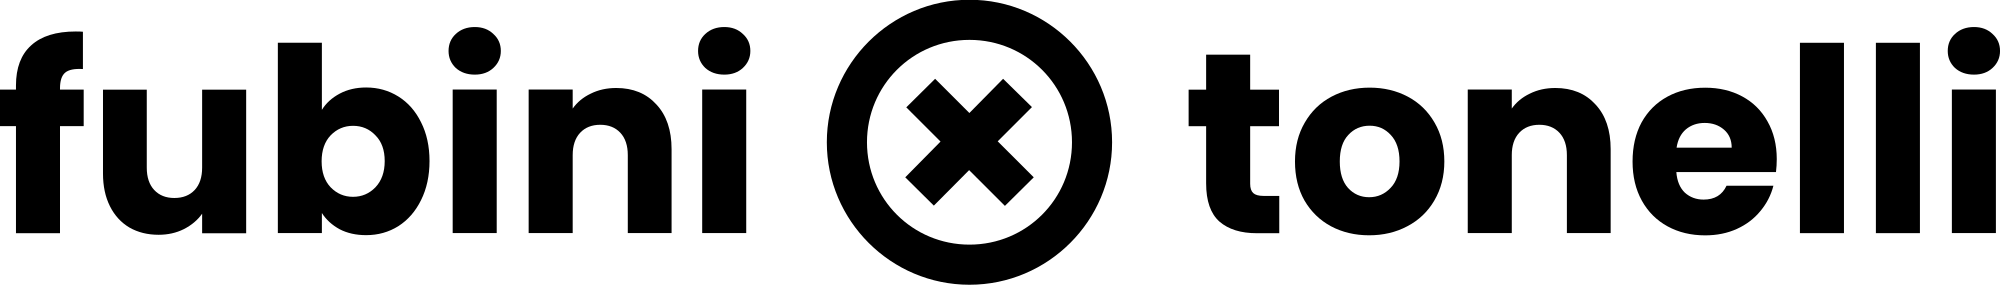
\includegraphics[width=0.38\textwidth]{img/Logo_s.png}}
\end{center}

\clearpage
\vspace*{\stretch{12}}
© Gli autori. Alcuni diritti riservati

Questa opera è rilasciata sotto licenza Creative Commons BY-NC-SA 4.0.\\
\url{https://creativecommons.org/licenses/by-nc-sa/4.0/}

In particolare, senza il permesso degli autori non è consentito fare copie di questo libro (né cartacee né digitali) per rivenderle.

Il codice sorgente \LaTeX \ è disponibile su \\
\url{https://github.com/fubinitonelli/probabilita}

\href{https://fubinitonelli.it}{\texttt{fubinitonelli.it}} - \href{mailto:info@fubinitonelli.it}{\texttt{info@fubinitonelli.it}}

\vspace*{\stretch{2}}

\textsc{Revisione del \today}
\IfFileExists{commit_hash.part}
{- \texttt{\input{commit_hash.part}}}
{}

\textsc{Developed with git 
\includegraphics[height=1em]{img/icons/code.pdf} by:}

\textsc{Fabrizio Bernardi} - \href{fabrizio@fubinitonelli.it}{\texttt{fabrizio@fubinitonelli.it}}\\
\textsc{Gioele Cerri} - \href{gioele@fubinitonelli.it}{\texttt{gioele@fubinitonelli.it}}\\
\textsc{Bruno Guindani} - \href{bruno@fubinitonelli.it}{\texttt{bruno@fubinitonelli.it}}\\
\textsc{Simone Polito} - \href{simone@fubinitonelli.it}{\texttt{simone@fubinitonelli.it}}\\
\textsc{Aron Wussler} - \href{aron@fubinitonelli.it}{\texttt{aron@fubinitonelli.it}}


\vspace{\stretch{5}}
\clearpage

\pagestyle{plain}


\hypersetup{linkcolor=black}

\pdfbookmark[1]{Indice}{index}
\setcounter{tocdepth}{2}
\tableofcontents
\hypersetup{linkcolor=blue}
\cleardoublepage

\pagestyle{inner}

\section{Catene di Markov}
In questo capitolo finale si vuole descrivere l'\emph{evoluzione di una grandezza} distribuita in maniera casuale e descritta da una famiglia di variabili aleatorie,
studiando quelli che verranno definiti come \emph{processi stocastici}.
In questo testo sarà trattata solo una sottoclasse di processi,
quella delle \emph{catene di Markov a tempo discreto}, nelle quali il valore futuro della grandezza dipende solamente dal valore attuale e non dalla storia dell'evoluzione.
Si studieranno quindi le leggi secondo cui una grandezza evolve da uno \textit{stato} (cioè un valore) ad un altro e le caratteristiche dei suddetti stati.

\subsection{Definizioni base}

\begin{defn}\label{proc-stoc}
	\index{processo stocastico}
	\index{stati, spazio degli}
	Un \textbf{processo stocastico} è una famiglia di VA $(X_t)_{t \in T}$, $X_t: \Omega \to E$,
	tutte definite sullo stesso spazio di probabilità $\Dom$, a valori nello stesso spazio misurabile $(E,\Ec)$,
	e dipendenti da un parametro $t \in T \subseteq \RR^+ = [0,+\infty)$. \\
	L'insieme $E$ è detto \textbf{spazio degli stati} e i suoi elementi \textbf{stati}.

\end{defn}
Il processo stocastico è una nozione generalizzata rispetto alle \textit{successioni} di VA trattate nei capitoli precedenti.
La principale differenza risiede nel fatto che in un processo stocastico il parametro $t$ appartiene a un generico insieme $T$ e quindi può anche essere \emph{continuo}, a differenza dell'indice $n \in \NN$ delle successioni (anche se, in questo capitolo, $T$ sarà spesso discreto per semplicità di trattazione).
Inoltre, il codominio delle VA è un generico spazio misurabile $(E,\Ec)$ e non necessariamente $\RR$.
Tipicamente, infine, il parametro $t$ rappresenta il \textit{tempo} della misurazione o dell'osservazione.

\begin{ese}
	Un esempio frequente di processo stocastico è una grandezza misurata ad istanti $t$ di tempo diversi.
	Consideriamo il caso del \emph{tempo discreto}, che descrive una \emph{evoluzione a scatti}:
	$$T \subseteq \ZZ^+ = \{0,\, 1,\, 2,\, \dots\}$$
	La $\sigma$-algebra del codominio è l'insieme delle parti $\Ec = 2^E$, con $E$ discreto.
\end{ese}

\begin{defn}\label{catena}
	\index{catena}
	Un processo stocastico si dice \textbf{catena} se il suo spazio degli stati $E$ è discreto.
\end{defn}

\begin{ese}
	L'esempio precedente è una catena, così come ogni \textit{successione} di VA della forma $X_n: \Omega \to E$,
	con $E$ discreto e $n \in \ZZ^+$, che d'ora in poi scriveremo come $n \ge 0$ per semplicità di notazione.
\end{ese}

\begin{ese}
	Sono catene a tempo discreto valide:
	\begin{itemize}
		\item il risultato dell'$n$-esimo lancio di una moneta che viene lanciata infinite volte,
		 	dove ciascun lancio avviene ad un preciso istante di tempo: $X_n: \Omega \to E = \{T, C\}$;
		\item il tempo metereologico a Milano dell'$n$-esimo giorno del 2019: $X_n: \Omega \to \{\text{sole},\, \text{pioggia},\, \dots\}$;
		\item il valore di un bit dopo la trasmissione attraverso l'$n$-esimo canale rumoroso: $X_n: \Omega \to \{0,1\}$;
		\item il capitale di un giocatore d'azzardo dopo l'$n$-esimo lancio di una moneta,
			che gli fa guadagnare se esce testa e gli fa perdere se esce croce: $X_n: \Omega \to \RR$.
	\end{itemize}
\end{ese}

\begin{figure}[H]

	\centering
	\(
	\vcenter{\hbox{\begin{tikzpicture}
		\begin{scope}
			\draw {(0, 0) rectangle (2,2)} node[below left] {\large $\Omega$};

			\node[circle,fill, label=$\omega_1$, scale=0.3] at (1.3,0.5) {};
			\node[circle,fill, label=$\omega_2$, scale=0.3] at (0.6,1) {};
		\end{scope}
	\end{tikzpicture}}}
	\)
	\hskip 50pt
	\(
	\vcenter{\hbox{\begin{tikzpicture}
	\begin{axis}[
	axis lines = middle,
	width=0.55\textwidth,
	height=0.40\textwidth,
	yticklabels={,,},
	xticklabels={,,},
	xlabel=$n$,
	ylabel=$X_n$
	]

	\draw [line width=0.4mm, color=lightblue] (axis cs:0.5,1.5) -- (axis cs:1.5,0.5) -- (axis cs:2.5,1.5) -- (axis cs:3.5,0.5) -- (axis cs:4.5,1.5);
  \draw [line width=0.4mm, color=black] (axis cs:0.5,0.5) -- (axis cs:1.5,1.5) -- (axis cs:2.5,0.5) -- (axis cs:3.5,1.5) -- (axis cs:4.5,0.5);

	\node[color=lightblue] at (axis cs:5.5, 1.5) {$X_n (\omega_1)$};
	\node at (axis cs:5.5, 0.5) {$X_n (\omega_2)$};

	\addplot [draw=none, forget plot] coordinates {(0,0)};
	\addplot [draw=none, forget plot] coordinates {(6.5,2)};

	\end{axis}
	\end{tikzpicture}}}
	\)
	\caption{catene $X_n$ rispetto a diversi stati iniziali $\omega_1$ e $\omega_2$}
\end{figure}

\index{traiettoria}
Fissando l'esito elementare $\omega \in \Omega$, si ottiene una \emph{traiettoria} nello spazio degli stati $E$,
ovvero una successione di valori $\{x_n\}_n = \{X_n(\omega)\}_n \subseteq E$. Chiaramente, fissando invece l'indice $n \ge 0$, si ottiene una singola VA $X_n: \Omega \to E$.

\begin{defn}\label{matrans}
	\index{matrice di transizione}
	\index{probabilità!di transizione}
	Una matrice $P = [p_{ij}]$ con $i,j \in E$ è detta \textbf{matrice di transizione} o \textbf{matrice stocastica} se:
	$$p_{ij} \ge 0 \ \forall i,j \in E \quad \text{e} \quad \sum_{j \in E} p_{ij} = 1 \enspace \forall i \in E$$
	In altre parole, la $i$-esima riga $p_{i \bigcdot}$ è una \emph{densità discreta} di probabilità su $E$, $\forall i \in E$.
	Ogni elemento $p_{ij}$ di questa matrice è detto \textbf{probabilità di transizione} da $i$ a $j$.
\end{defn}

L'intuizione suggerisce che $p_{ij}$ sia effettivamente la probabilità, partendo dallo stato $i$ di spostarsi nello stato $j$ in un unico passo.
Questo significato sarà verificato formalmente più avanti.
Nel frattempo, rafforzeremo l'intuizione sul modello di catena a tempo discreto mediante alcuni esempi.

\needspace{3\baselineskip}
\begin{ese}~\\
	\label{catene-triangolari}
	\begin{enumerate}
		\item Sia $E = \{1,2\}$. Dati $p,q \in [0,1]$, un esempio di matrice di transizione è la seguente:
		$$P = \begin{bmatrix} 1-p & p \\ q & 1-q\end{bmatrix}$$
		Intuitivamente, questo significa che il sistema descritto da $P$ ha, in ogni istante di tempo $n\ge 0$, due stati possibili, detti 1 e 2.
		Le probabilità sono così distribuite:
		\begin{itemize}[label=$\ast$]
			\item $p$ indica la probabilità che lo stato passi da 1 a 2 in un determinato istante di tempo;
			\item $q$ che lo stato passi da 2 a 1;
			\item $1-p$ che lo stato rimanga in 1;
			\item $1-q$ che lo stato rimanga in 2.
		\end{itemize}

		\begin{figure}[H]
		  \centering
		  \begin{tikzpicture}
		    \begin{scope}
					\node[circle,fill, label=$1$, scale=0.3] at (0,0) {};
					\node[circle,fill, label=$2$, scale=0.3] at (3,0) {};

			    \node at (0.1,0.1) {} edge[->, line width=0.4mm, looseness=1, bend left=20]  (2.8, 0.1) ; % da 1 a 2
					\node at (2.9,-0.1) {} edge[->, line width=0.4mm, looseness=1, bend left=20]  (0.2, -0.1); % da 2 a 1

					\node at (1.5, 0.6) {$p$};
					\node at (1.5, -0.6) {$q$};

					\node at (-0.1,-0.1) {} edge[->, line width=0.4mm, looseness=8, bend left=125]  (-0.18, 0.1) ; % da 1 a 1
					\node at (3.1,0.1) {} edge[->, line width=0.4mm, looseness=8, bend left=125]  (3.18, -0.1) ; % da 2 a 2

					\node at (-1.3, 0) {$1-p$};
					\node at (4.3, 0) {$1-q$};

		    \end{scope}
		  \end{tikzpicture}
		  \caption{illustrazione della catena dell'esempio 1}
		\end{figure}

		\item Dato un sistema a tre stati $E=\{1,2,3\}$, che varia secondo un tempo discreto $n \ge 0$, si può avere la seguente matrice di transizione:
			$$P = \begin{bmatrix} 0 & 1 & 0 \\ 0 & \nicefrac 1 2 & \nicefrac 1 2 \\ \nicefrac 1 2 & 0 & \nicefrac 1 2\end{bmatrix}$$
		Il sistema non può compiere tutte le transizioni possibili.
		Per esempio, non può ripercorrere al contrario il ``ciclo'' $1\to2\to3$: può solo andare avanti o, nel caso si trovi in 2 o in 3, rimanere nello stesso stato.
		Questo perché la probabilità di spostarsi da 3 a 2 (in un unico passo) è nulla: $p_{32} = 0$.
		Si noti, comunque, che questo \textit{non} impedisce il ritorno da 3 a 2 in $n \ge 2$ passi mediante passaggi intermedi in altri stati (in questo caso, 1).

		\begin{figure}[H]
		  \centering
		  \begin{tikzpicture}
		    \begin{scope}
					\node[circle,fill, label=$2$, scale=0.3] at (0,0) {};
					\node[circle,fill, label=$3$, scale=0.3] at (3,0) {};
					\node[circle,fill, label=$1$, scale=0.3] at (1.5, 2.598) {};

			    \node at (0.1,0) {} edge[->, line width=0.4mm]  (2.8,0) ; % da 1 a 2
					\node at (2.9,0.1) {} edge[->, line width=0.4mm]  (1.6,2.4); % da 2 a 3
					\node at (1.43, 2.5) {} edge[->, line width=0.4mm]  (0.15, 0.2); % da 3 a 1

					\node at (1.5, -0.35) {$\frac{1}{2}$};
					\node at (2.45, 1.4) {$\frac{1}{2}$};
					\node at (0.55, 1.4) {$1$};

					\node at (-0.1,-0.1) {} edge[->, line width=0.4mm, looseness=8, bend left=125]  (-0.18, 0.1) ; % da 1 a 1
					\node at (3.1,0.1) {} edge[->, line width=0.4mm, looseness=8, bend left=125]  (3.18, -0.1) ; % da 2 a 2

					\node at (-1, 0) {$\frac{1}{2}$};
					\node at (4, 0) {$\frac{1}{2}$};

		    \end{scope}
		  \end{tikzpicture}
		  \caption{illustrazione della catena dell'esempio 2}
		\end{figure}

		\item Considerando ancora $E=\{1,2,3\}$ un'altra matrice può essere:
		$$P = \begin{bmatrix} 0 & 1 & 0 \\ 1 & 0 & 0 \\ 0 & 0 & 1\end{bmatrix}$$
		Questo sistema possiede due ``sottosistemi'' che non comunicano: partendo da 1 si può solo passare a 2 e viceversa,
		mentre partendo da 3 non si può che rimanere per sempre in 3.
		L'evoluzione, in questo caso, è quindi parzialmente ``deterministica'', cioè si possono effettuare alcune previsioni conoscendo lo stato di partenza.

		\begin{figure}[H]
		  \centering
		  \begin{tikzpicture}
		    \begin{scope}
					\node[circle,fill, label=$1$, scale=0.3] at (0,0) {};
					\node[circle,fill, label=$2$, scale=0.3] at (3,0) {};
					\node[circle,fill, label=$3$, scale=0.3] at (1.5, 2.598) {};

					\node at (0.1,0.1) {} edge[->, line width=0.4mm, looseness=1, bend left=20]  (2.8, 0.1) ; % da 1 a 2
 				 	\node at (2.9,-0.1) {} edge[->, line width=0.4mm, looseness=1, bend left=20]  (0.2, -0.1); % da 2 a 1

				 	\node at (1.5, 0.6) {$1$};
				 	\node at (1.5, -0.6) {$1$};
					\node at (1.6, 2.5) {} edge[->, line width=0.4mm, looseness=8, bend left=125] (1.35,2.42) ; % da 3 a 3
					\node at (1.5, 1.4) {$1$};

		    \end{scope}
		  \end{tikzpicture}
		  \caption{illustrazione della catena dell'esempio 3}
		\end{figure}

	\end{enumerate}
\end{ese}

\begin{defn}\label{cat-mark}
	\index{catena di Markov}
	\index{Markov!catena di}
	\index{Markov!proprietà di}
	\index{omogeneità (catene di Markov)}
	\index{legge!iniziale (catene di Markov)}
	Dati uno spazio di probabilità $\Dom$ e uno spazio misurabile $(E, 2^E)$, una famiglia di VA $X_n: \Omega \to E$,
	con $n \ge 0$, è detta \textbf{catena di Markov omogenea} a valori in $E$ di \textbf{legge iniziale} $v$ e
	\textbf{matrice di transizione} $P = [p_{ij}]$, con $i,j \in E$, se:
	\begin{enumerate}
		\item $X_0 \sim v$;
		\index{proprietà di Markov}
		\item $\forall n \ge 0$ e $\forall i,j \in E$, si ha la \textbf{proprietà di Markov}: \\
		$$\PP(X_{n+1} = j |
		X_n=i, X_{n-1}=i_{n-1},\dots,X_0=i_0) =
		\PP(X_{n+1} = j | X_n = i)$$
		qualora le suddette probabilità condizionate esistano;
		\item vale la proprietà di \textbf{omogeneità}: $$\PP(X_{n+1} = j | X_n = i) = p_{ij} \enspace \forall i,j \in E$$
		ovvero la probabilità di transizione \emph{non} dipende da $n$.
	\end{enumerate}
	Per indicare una catena di Markov omogenea definita come sopra useremo la notazione compatta $(X_n)_{n \ge 0} \ \markov(v,P)$.
\end{defn}
\subsubsection{Interpretazione}
La proprietà di Markov afferma che, quando si conosce il valore \emph{presente} di una VA ($X_n = i$)
e si vuole fare una stima sul valore \emph{futuro} (nell'istante di tempo successivo) di quella VA ($X_{n+1} = j$), conoscere i valori
\emph{passati} di quella VA $(X_{n-1} = i_{n-1}, \dots, X_0 = i_0)$ non fornisce alcuna informazione aggiuntiva
rispetto al conoscere il valore presente.
In altre parole, noti lo stato attuale e l'istante di osservazione di una catena di Markov, \textbf{il prossimo valore} assunto dalla catena \textbf{dipende solo dal valore attuale}.
Tale proprietà è confermata dall'intuizione per alcuni tipi di fenomeno: per esempio, se un processo
stocastico indica la posizione nello spazio di una particella e la sua velocità, è naturale pensare
che i dati attuali siano sufficienti per cercare di prevedere la sua posizione nel successivo istante di tempo, senza bisogno di conoscere la sua storia.

Si noti, comunque, che questa proprietà \emph{non} significa che i valori futuri sono indipendenti dai valori passati, perché queste caratteristiche di ``quasi-indipendenza'' richiedono la conoscenza dello stato attuale\footnote{Vedremo infatti che la conoscenza dell'istante di osservazione non è necessaria per formulare previsioni sull'evoluzione di una catena di Markov omogenea.}, che a seconda del modello preso in esame può anche non essere accessibile.
È bene infatti rimarcare che le variabili $X_n$ della catena \emph{non sono indipendenti} tra loro né tantomeno identicamente distribuite.

Si noti, infine, che in una catena di Markov è cruciale la scelta di due elementi: la \emph{VA osservata} $X_n$ e lo \emph{spazio degli stati} $E$.
Nell'esempio precedente della particella, la sola posizione non è un'informazione sufficiente per formulare la previsione, e servirebbero informazioni aggiuntive dal suo passato.
%Data una catena di Markov e ricavata la sua matrice di transizione $P$, che corrisponde a una \emph{legge di evoluzione} della grandezza, si può andare a ritroso e ricavare anche la legge iniziale $v$. %Questa frase è inutile e un non sequitur (Br1)

\subsection{Esempi notevoli}\label{rovina-gioc}
	\index{rovina del giocatore}
	Introduciamo ora due esempi particolarmente significativi di catene di Markov, che saranno ripresi più volte nel corso della trattazione dell'argomento: la rovina del giocatore e l'urna di Ehrenfest.
	\begin{ese}[rovina del giocatore] 
		% Non mi piace molto l'utilizzo di ese qui. Idem sotto con l'urna. Idee? (Br1)
		% Lo lascerei per coerenza con il resto degli esempi (AW)
		Immaginiamo due giocatori, Aron e Bruno hanno ciascuno un capitale iniziale, rispettivamente $a, b \in \NN$.
		Ad ogni istante di tempo viene lanciata una moneta, che ha probabilità $p$ di risultare testa, e possono accadere due eventi: se esce testa, Aron riceve 1 da Bruno; se esce croce invece Bruno riceve 1 da Aron.
		I lanci di moneta continuano fino a che uno dei due giocatori non entra in rovina esaurendo il suo capitale.
		
		Il numero totale di lanci effettuati prima della rovina di uno dei due giocatori è casuale e incognito a priori.
		Una formulazione equivalente del gioco è che i lanci proseguano anche dopo la rovina di uno dei due giocatori, ma da quel momento in poi non ci siano più scambi di denaro.
		Questo permette di operare con le catene di Markov, in quanto si ha un numero infinito di lanci, ovvero di VA.
		
		Sia dunque $X_n$ il capitale di Aron dopo l'$n$-esimo lancio.
		Grazie al cambio di formulazione sopra discusso si ha $T = \ZZ^+$.
		Inoltre $E = \{0,1,\dots,a+b\}$, in quanto un giocatore può possedere al massimo la somma dei due capitali,
		e $v = \delta_a$, in quanto si suppone deterministicamente che Aron inizi sempre il gioco con capitale $a$.
		La matrice di transizione è tridiagonale, eccetto che per la prima e l'ultima riga, in quanto una volta raggiunta la rovina si rimane per sempre in quello stato con probabilità 1:
		$$P = \begin{bmatrix}
		1   & 0 & 0 & 0 & \dots \\
		1-p & 0 & p & 0 & \dots \\
		0 & 1-p & 0 & p & \dots \\
		&& \ddots & \ddots & \ddots \\
		& \dots & 0 & 1-p & 0 & p \\
		& \dots & 0 & 0 & 0 & 1
		\end{bmatrix}$$
		
		\begin{figure}[H]
			\centering
			\begin{tikzpicture}
			\begin{scope}
			\node[circle,fill, label=$0$, scale=0.3] at (0,0) {};
			\node[circle,fill, label=$1$, scale=0.3] at (2,0) {};
			\node[circle,fill, label=$2$, scale=0.3] at (4,0) {};
			\node[circle,fill, scale=0.3] at (6,0) {};
			%\node at (6, 0.5) {$a+b-1$};
			\node[circle,fill, scale=0.3] at (8,0) {};
			\node at (8, 0.5) {$a+b$};
			
			\node at (-1, 0) {$1$};
			\node at (-0.1,-0.1) {} edge[->, line width=0.4mm, looseness=8, bend left=125]  (-0.18, 0.1) ; % da 0 a 0
			
			\node at (1.9,-0.1) {} edge[->, line width=0.4mm, looseness=1, bend left=20]  (0.2, -0.1); % da 1 a 0
			\node at (1, -0.6) {$1-p$};
			
			\node at (2.1,0.1) {} edge[->, line width=0.4mm, looseness=1, bend left=20]  (3.8, 0.1) ; % da 1 a 2
			\node at (3.9,-0.1) {} edge[->, line width=0.4mm, looseness=1, bend left=20]  (2.2, -0.1); % da 2 a 1
			\node at (3, 0.6) {$p$};
			\node at (3, -0.6) {$1-p$};
			
			\node at (4.1,0.1) {} edge[->, line width=0.4mm, looseness=1, bend left=20, dashed]  (5.8, 0.1) ; % da 1 a 2
			\node at (5.9,-0.1) {} edge[->, line width=0.4mm, looseness=1, bend left=20, dashed]  (4.2, -0.1); % da 2 a 1
			
			\node at (5, 0.6) {$p$};
			\node at (5, -0.6) {$1-p$};
			\node at (5, 0) {$\dots$};
			
			\node at (6.1,0.1) {} edge[->, line width=0.4mm, looseness=1, bend left=20]  (7.8, 0.1) ; % da a+b-1 a a+b
			\node at (7, 0.6) {$p$};
			
			\node at (8.1,0.1) {} edge[->, line width=0.4mm, looseness=8, bend left=125]  (8.18, -0.1) ; % da a+b a a+b
			\node at (9, 0) {$1$};
			
			\end{scope}
			\end{tikzpicture}
			\caption{rovina del giocatore}
		\end{figure}
	\end{ese}
	

\begin{ese}[urna di Ehrenfest] \label{urna-ehren}
	\index{urna di Ehrenfest}
	Forniamo due formulazioni equivalenti del problema:
	\begin{itemize}
		\item si ha un'urna contenente $N$ palline, di colore bianco oppure nero. Ad ogni istante di tempo si estrae una pallina a caso (con legge uniforme),
			la si sostituisce con una del colore opposto e la si rimette nell'urna. Qui $X_n$ è il numero di palline nere dopo l'$n$-esima estrazione.
		\item si ha un sistema chiuso formato da 2 recipienti comunicanti, $A$ e $B$, che contiene in totale $N$ molecole di gas.
			Ad ogni istante di tempo, una molecola a caso (con legge uniforme) nel sistema si trasferisce dal recipiente in cui si trova, nell'altro recipiente.
			Qui $X_n$ è il numero di molecole nel recipiente $A$ dopo l'$n$-esimo istante di tempo.
	\end{itemize}
	In entrambi i casi $E = \{0,1,\dots,N\}$, $T = \ZZ^+$ (similmente all'esempio precedente), e la proprietà di Markov è soddisfatta.
	Anche qui abbiamo una matrice tridiagonale, questa volta incluse la prima e l'ultima riga, ma con probabilità variabile a seconda dello stato.
	Per esempio, la probabilità di passare da 2 a 1 palline nere (o molecole nel recipiente $A$) è pari alla probabilità che venga pescata una delle 2 su un totale di $N$; ovvero, $p_{21} = \frac 2 N$, e così via per tutte le altre probabilità di transizione.
	La matrice di transizione risultante è la seguente:
	$$P = \begin{bmatrix}
	0 & 1 & 0 & 0 & \dots \\
	\frac 1 N & 0 & \frac{N-1}N & 0 & \dots \\
	0 & \frac 2 N & 0 & \frac{N-2}N & \dots \\
	&& \ddots & \ddots & \ddots \\
	& \dots & 0 & \frac{N-1}N & 0 & \frac 1 N \\
	& \dots & 0 & 0 & 1 & 0
	\end{bmatrix}$$
\end{ese}
\begin{figure}[H]
	\centering
	\begin{tikzpicture}
		\begin{scope}
			\node[circle,fill, label=$0$, scale=0.3] at (0,0) {};
			\node[circle,fill, label=$1$, scale=0.3] at (2,0) {};
			\node[circle,fill, label=$2$, scale=0.3] at (4,0) {};
			\node[circle,fill, scale=0.3] at (6,0) {};
			\node at (6, 0.4) {$N-2$};
			\node[circle,fill, scale=0.3] at (8,0) {};
			\node at (8, 0.4) {$N-1$};
			\node[circle,fill, label=$N$, scale=0.3] at (10,0) {};

			\node at (0.1,0.1) {} edge[->, line width=0.4mm, looseness=1, bend left=20]  (1.8, 0.1) ; % da 0 a 1
			\node at (1.9,-0.1) {} edge[->, line width=0.4mm, looseness=1, bend left=20]  (0.2, -0.1); % da 1 a 0
			\node at (1, 0.6) {$1$};
			\node at (1, -0.6) {$\frac{1}{N}$};

			\node at (2.1,0.1) {} edge[->, line width=0.4mm, looseness=1, bend left=20]  (3.8, 0.1) ; % da 1 a 2
			\node at (3.9,-0.1) {} edge[->, line width=0.4mm, looseness=1, bend left=20]  (2.2, -0.1); % da 2 a 1
			\node at (3, 0.6) {$\frac{N-1}{N}$};
			\node at (3, -0.6) {$\frac{2}{N}$};

			\node at (4.1,0.1) {} edge[->, line width=0.4mm, looseness=1, bend left=20, dashed]  (5.8, 0.1) ; % da 1 a 2
			\node at (5.9,-0.1) {} edge[->, line width=0.4mm, looseness=1, bend left=20, dashed]  (4.2, -0.1); % da 2 a 1
			\node at (5, 0) {$\dots$};

			\node at (6.1,0.1) {} edge[->, line width=0.4mm, looseness=1, bend left=20]  (7.8, 0.1) ; % da N-2 a N-1
			\node at (7.9,-0.1) {} edge[->, line width=0.4mm, looseness=1, bend left=20]  (6.2, -0.1); % da N-1 a N-2
			\node at (7, 0.6) {$\frac{2}{N}$};
			\node at (7, -0.6) {$\frac{N-1}{N}$};

			\node at (8.1,0.1) {} edge[->, line width=0.4mm, looseness=1, bend left=20]  (9.8, 0.1) ; % da N-1 a N
			\node at (9.9,-0.1) {} edge[->, line width=0.4mm, looseness=1, bend left=20]  (8.2, -0.1); % da N a N-1
			\node at (9, 0.6) {$\frac{1}{N}$};
			\node at (9, -0.6) {$1$};

		\end{scope}
	\end{tikzpicture}
	\caption{urna di Ehrenfest}
\end{figure}

\subsection{Leggi congiunte}
Data una catena $(X_n)_{n \ge 0} \ \markov(v,P)$, per definizione $X_0 \sim v$ e quindi si ha che:
$$X_1 | (X_0 = i) \sim p_{i\bigcdot} \text{ in quanto } \PP(X_0 = i) = v_i \text{ e } \PP(X_1 = j | X_0 = i) = p_{ij}$$
Pertanto, grazie alle proprietà della legge condizionata (capitolo \ref{section-leggi-condizionate}):
$$\PP(X_0 = i, X_1 = j) = \PP(X_0 = i) \ \PP(X_1 = j | X_0 = i) = v_i \ p_{ij}$$
Si può dunque constatare che conoscendo la legge marginale di $X_0$ e la legge condizionata di $X_1|X_0$, è nota anche la legge congiunta di $(X_0, X_1)$.
Questa ``concatenazione'' di leggi mediante un prodotto\footnote{Questa proprietà e altre simili (anche viste in altri capitoli di questo testo) che permettono di ricavare una legge congiunta dal prodotto di altre leggi sono incluse nella categoria delle cosiddette \emph{leggi della catena.}}
funziona anche per ottenere la legge congiunta di un numero qualsiasi di VA della catena:

\begin{teo}\label{teo-legge-mark}
	Sia $(X_n)_{n \ge 0} \ \markov(v,P)$. Allora, $\forall n \ge 0$ e $\forall i_0,\dots,i_n \in E$, si ha:
	$$ \PP(X_0=i_0, \, X_1=i_1, \, \dots, \, X_n=i_n) =
	v_{i_0} \ \, p_{i_0 i_1} \ \, p_{i_1 i_2} \ \, \cdots \ \, p_{i_{n-1} i_n} $$
\end{teo}
\needspace{2\baselineskip}
\begin{dimo}~
	\begin{enumerate}
		\item Si supponga $\PP(X_0 = i_0, \dots, X_n = i_n) > 0$. \\
		Usando al contrario la definizione di probabilità condizionata sugli eventi $(X_n = i_n)$ e $(X_0 = i_0, \dots, X_{n-1} = i_{n-1})$ si ha che:
			\begin{align*}
				\PP(X_0 &= i_0, \, \dots, \, X_n = i_n) \\
				= \, & \PP(X_n = i_n | X_{n-1} = i_{n-1}, \dots, X_0 = i_0) \ \PP (X_{n-1} = i_{n-1}, \dots, X_0 = i_0) \\
				= \, & p_{i_{n-1} i_n} \ \PP (X_{n-1} = i_{n-1}, \dots, X_0 = i_0) &\mathmakebox[1pt][r]{\hfill\text{(per la pr. Markov)}} \\
				= \, & p_{i_{n-1} i_n} \ \PP(X_{n-1}=i_{n-1} | X_{n-2}=i_{n-2},\dots,X_0=i_0) \cdot\\
				  &\cdot \PP(X_{n-2}=i_{n-2},\dots,X_0=i_0) \\
				= \, & \dots &\mathmakebox[1pt][r]{\hfill\text{(ripetendo $n$ volte)}} \\
				= \, & p_{i_{n-1} i_n} \ \cdots \ p_{i_1 i_0} \ v_{i_0}
			\end{align*}
		\item Il caso $\PP(X_0 = i_0, \dots, X_n = i_n) = 0$ è un utile esercizio per il lettore.\footnote{Dimostrazione del lettore quotata a 1.1} \qedhere
	\end{enumerate}
\end{dimo}

Questo teorema mostra come l'evoluzione del fenomeno dipenda fortemente dalla legge iniziale.
È dunque impensabile cercare di studiare l'evoluzione di una grandezza al variare di $v$ e
tenendo fissa la matrice di transizione $P$, perché cambierebbero tutte le leggi congiunte
creando quindi altre catene di Markov diverse e slegate tra loro.
Si dice dunque che la catena di Markov è definita dai due \emph{parametri} $P$ e $v$:
ciò è evidenziato dalla notazione compatta scelta per indicarle.

Il caso $v \not\sim \delta$ indica una situazione iniziale non deterministica e non nota a priori,
per esempio il caso in cui l'inizio della catena sia il prodotto di un altro esperimento aleatorio avvenuto precedentemente.

Introduciamo ora una notazione largamente utilizzata per la sua brevità: si indichi con $\PP_i(\bigcdot)$ la probabilità $\PP(\bigcdot | X_0 = i)$, quindi sottintendendo che è noto lo stato iniziale $i$ della catena.

\begin{coro}\label{coro-mark}
	Sia $(X_n)_{n \ge 0} \ \markov(v,P)$ sullo spazio di probabilità $\Dom$.
	Siano inoltre $v_i = \PP(X_0=i) > 0 \enspace \forall i$ e $\PP_i(A) = \PP(A | X_0=i) \enspace \forall A \in \Ac$.
	Allora $(X_n)_{n \ge 0}$ è $\markov(v,P)$ anche sullo spazio di probabilità $(\Omega,\Ac,\PP_i)$.
\end{coro}
Ciò non è scontato, perché in generale sostituendo $\PP$ con una legge qualsiasi non si ha alcuna garanzia sul fatto che si ottenga ancora una catena di Markov.
Il risultato permette di semplificare i conti e la notazione quando è nota la legge iniziale, di fatto ``incorporando'' la situazione iniziale direttamente nella legge di probabilità della catena.
Vedremo che un risultato simile vale anche se $v \sim \delta$ (quindi anche con componenti nulle di $v$). \\

\subsubsection{Notazione matriciale}
Si identifichi ora ogni densità $\pi$ di probabilità discreta su $E$ con un \emph{vettore riga} di componenti $\pi_i$, $i \in E$, con $\pi_i \ge 0 \enspace \forall i$ e $\sum_i \pi_i = 1$.
Si introduca il vettore riga $\pi P$, tale che:
$$(\pi P)_j = \sum_i \pi_i p_{ij} \ \forall j \in E$$
Infine, si introducano anche la matrice $P^2$, tale che:
$$(P^2)_{ij} = \sum_k p_{ik} p_{kj} \ \forall i,j \in E$$
Analogamente le altre potenze $P^n$ di $P$, con $n \ge 0$. \\
Indicheremo con $p_{ij}^{(n)}$ l'elemento in posizione $(i,j)$ della matrice $P^n$; dunque:
$$P^n = \left[ p_{ij}^{(n)} \right]_{i,j \in E}$$
Similmente denoteremo con $v^{(n)}$ la legge della VA $X_n$: si ha dunque $X_n \sim v^{(n)}$ e $v^{(0)} = v$. \\

\begin{teo}\label{teo-vettori-mark}
	Sia $(X_n)_{n \ge 0} \ \markov(v,P)$.
	Allora:
	\begin{enumerate}[label=(\roman*)]
		\item $v^{(n)} = v^{(0)} P^n \ \forall n \ge 0$, ovvero in componenti:
		 	$$\PP(X_n = j) = (v P^n)_j \ \forall n \ge 0, j \in E$$
		\item vale la seguente uguaglianza, ammesso che le probabilità condizionate ivi utilizzate esistano:
			$$p_{ij}^{(n)} = \PP(X_{m+n} = j | X_m = i) = \PP(X_n = j | X_0 = i) \ \forall m,n \ge 0, \ i,j \in E$$
		\item per ogni $k, n_1,\dots,n_k \ge 0, \ i_1,\dots,i_k \in E$,
		$$\PP(X_{n_1}=i_1, \, \dots, X_{n_k}=i_k) = \sum_{i_0 \in E} \ v_{i_0} \ p_{i_0 i_1}^{(n_1)} \
		p_{i_1 i_2}^{(n_2-n_1)} \ \cdots \ p_{i_{k-1} i_k}^{(n_k - n_{k-1})}$$
	\end{enumerate}
\end{teo}

Nel punto (ii), $p_{ij}^{(n)}$ è la probabilità di transizione di $n$ passi partendo dal tempo $m$;
in questo caso quindi la matrice di transizione del passaggio è proprio $P^{(n)}$, e tale passaggio \emph{non dipende dall'istante temporale $m$ di partenza}!
Questo è un effetto dell'omogeneità (temporale, cioè in $n$) della catena di Markov: le previsioni sul valore di $X_n$ non dipendono dal tempo di osservazione, ma solo dallo stato in cui la catena si trova attualmente. \\
Inoltre, il punto (i) rappresenta una \emph{formula delle probabilità totali} rispetto ai valori di $X_0$:
$$\PP(X_n=j) = \sum_{i \in E} \PP(X_n=j, X_0=i) = \sum_{i \in E} \PP(X_n=j | X_0=i) \, \PP(X_0=i)$$
$$\implies \quad \PP(X_n=j) = \sum_{i \in E} v_i \, p_{ij}^{(n)}$$
dove $p_{ij}^{(n)}$ è la probabilità di passare da $i$ a $j$ in esattamente $n$ passi.
% Qualcuno mi controlla sta cosa? il (ii) sopra l'= non c'era ma non sapevo come altro giustificarlo (Br1)
% L'ho tolto, era così per definizione (SSL)

\begin{dimo}~
	\begin{enumerate}[label=(\roman*)]
		\item Fattorizzando le probabilità e grazie alla definizione di $P^n$:
	 	\begin{align*}
			\PP(X_n = j) &\ = \sum_{i_0,\dots,i_{n-1}} \PP(X_n=j, X_{n-1}=i_{n-1},\dots,X_0=i_0) \\
			&\stackrel{\ref{teo-legge-mark}}{=} \sum_{i_0,\dots,i_{n-1}} v_{i_0} \ p_{i_0 i_1} \ \dots \ p_{i_{n-2} i_{n-1}} \ p_{i_{n-1} j} \\
			&\ = (v P^n)_j
		\end{align*}
		\item In caso $m=0$ e $v=\delta_i$, l'uguaglianza $p_{ij}^{(n)} = \PP(X_n=j | X_0=i)$ è
			automaticamente soddisfatta per il punto (i).
		\item Si dimostra, a titolo di esempio, un caso particolare con sottovettore appartenente a un vettore di 9 componenti:
		\begin{align*}
			&\PP(X_3=i_3, X_5=i_5, X_9=i_9) =
			\sum_{\substack{i_0,i_1,i_2,i_4,\\i_6,i_7,i_8}} \PP(X_0=i_0,\dots,X_9=i_9) \\
			= &\sum v_{i_0} \ p_{i_0 i_1} \dots p_{i_8 i_9} \\
			= &\sum_{i_0} v_{i_0} \ \sum_{i_1,i_2} p_{i_0 i_1} \ p_{i_1 i_2} \ p_{i_2 i_3}
			\ \sum_{i_4} p_{i_3 i_4} \ p_{i_4 i_5} \ \sum_{i_6,i_7,i_8} \ p_{i_5 i_6} \ p_{i_6 i_7} \ p_{i_7 i_8} \ p_{i_8 i_9} \\
			= &\sum_{i_0} v_{i_0} \ p_{i_0 i_3}^3 \ p_{i_3 i_5}^2 \ p_{i_5 i_9}^4
			\stackrel{\text{(ii)}}{=} \sum_{i_0} v_{i_0} \ p_{i_0 i_3}^{(3)} \ p_{i_3 i_5}^{(2)} \ p_{i_5 i_9}^{(4)}
		\end{align*}
	\item[(ii)] Siano ora $m \ge 1$ e $\PP(X_m=i)>0$:
	\begin{align*}
		\PP(X_{m+n}=j | X_m=i) &= \frac{\PP(X_m=i, X_{m+n}=j)}{\PP(X_m=i)} \stackrel{\text{(iii)}}{=}
		\frac{\sum_{i_0} v_{i_0} \ p_{i_0 i}^{(m)} \ p_{ij}^{(n)}}{\sum_{i_0} v_{i_0} \ p_{i_0 i}^{(m)}} \\
		&= \frac{p_{ij}^{(n)} \sum_{i_0} v_{i_0} \ p_{i_0 i}^{(m)}}{\sum_{i_0} v_{i_0} \ p_{i_0 i}^{(m)}} =
		p_{ij}^{(n)}&\qedhere
	\end{align*}
	\end{enumerate}
\end{dimo}


\begin{teo}[equazione di Chapman-Kolmogorov]
	\index{Chapman-Kolmogorov, equazione di}
	$$\PP(X_{n+m}=j | X_0=i) = \sum_{l \in E} \PP(X_{n+m}=j | X_m=l) \ \PP(X_m=l | X_0=i)$$
\end{teo}
Scelto un istante $m$, si possono dunque elencare tutte gli stati $l$ che la catena di Markov può assumere in $m$, ovvero tutti i possibili ``percorsi'' osservati all'istante $m$, ed usarli per calcolare la probabilità di arrivare in $j$.
Mediante un'accorta scelta di $m$, spesso questo calcolo si semplifica enormemente grazie ad eventuali percorsi che hanno probabilità nulla e ad altre peculiarità della catena analizzata.

\begin{figure}[H]
  \centering
  \begin{tikzpicture}
  \begin{axis}[
    axis lines = middle,
    ylabel = $E$,
    xlabel = $n$,
    width=0.7\textwidth,
    height=0.5\textwidth,
    yticklabels={,,},
    xticklabels={,,}
  ]

  \addplot [draw=none, forget plot] coordinates {(-0.2, -0.9)};
	\addplot [draw=none, forget plot] coordinates {(2.4, 0.9)};

	%etichette
	\node at (axis cs:-0.1, 0.5) {$i$};
	\node at (axis cs:-0.1, -0.5) {$j$};
	\node at (axis cs:1, 0.13) {$m$};
	\node at (axis cs:2, 0.13) {$m+n$};

	%linee tratteggiate
	\draw [line width=0.2mm, dashed] (axis cs:0,-0.5) -- (axis cs:2, -0.5) -- (axis cs:2, 0);
	\draw [line width=0.2mm, dashed] (axis cs:1,-1) -- (axis cs:1,0.08);
	\draw [line width=0.2mm, dashed] (axis cs:1,0.18) -- (axis cs:1,1);

	%tacchette
	\draw [line width=0.2mm] (axis cs:0.95,0.7) -- (axis cs:1.05,0.7);
	\draw [line width=0.2mm] (axis cs:0.95,0.55) -- (axis cs:1.05,0.55);
	\draw [line width=0.2mm] (axis cs:0.95,0.4) -- (axis cs:1.05,0.4);
	\draw [line width=0.2mm] (axis cs:0.95,0.25) -- (axis cs:1.05,0.25);
	\draw [line width=0.2mm] (axis cs:0.95,-0.1) -- (axis cs:1.05,-0.1);
	\draw [line width=0.2mm] (axis cs:0.95,-0.3) -- (axis cs:1.05,-0.3);
	\draw [line width=0.2mm] (axis cs:0.95,-0.5) -- (axis cs:1.05,-0.5);
	\draw [line width=0.2mm] (axis cs:0.95,-0.7) -- (axis cs:1.05,-0.7);

	%linee
	\draw [line width=0.2mm, color=lightblue] (axis cs:0,0.5) -- (axis cs:1, 0.7) -- (axis cs:2, -0.5);
	\draw [line width=0.2mm, color=lightblue] (axis cs:0,0.5) -- (axis cs:1, 0.55) -- (axis cs:2, -0.5);
	\draw [line width=0.2mm, color=lightblue] (axis cs:0,0.5) -- (axis cs:1, 0.4) -- (axis cs:2, -0.5);
	\draw [line width=0.2mm, color=lightblue] (axis cs:0,0.5) -- (axis cs:1, 0.25) -- (axis cs:2, -0.5);
	\draw [line width=0.2mm, color=lightblue] (axis cs:0,0.5) -- (axis cs:1, -0.1) -- (axis cs:2, -0.5);
	\draw [line width=0.2mm, color=lightblue] (axis cs:0,0.5) -- (axis cs:1, -0.3) -- (axis cs:2, -0.5);
	\draw [line width=0.2mm, color=lightblue] (axis cs:0,0.5) -- (axis cs:1, 0.5) -- (axis cs:2, -0.5);
	\draw [line width=0.2mm, color=lightblue] (axis cs:0,0.5) -- (axis cs:1, -0.7) -- (axis cs:2, -0.5);
  \end{axis}
  \end{tikzpicture}
  \caption{Chapman-Kolmogorov: si calcolano tutti gli stati intermedi nell'istante $m$, sfruttandoli per calcolare la probabilità di arrivare in $j$.}
\end{figure}

\begin{dimo}
	Dall'algebra delle matrici ricordiamo che $P^{m+n} = P^m P^n$, e in particolare:
	$$p_{ij}^{(n+m)} = \sum_{l \in E} p_{il}^{(m)} \ p_{lj}^{(n)} \quad \forall i,j \in E$$
	L'equazione non è altro che la riscrittura di quest'ultima formula, tenuto conto del punto (ii) del teorema \ref{teo-vettori-mark}.
\end{dimo}

\begin{teo}\label{teo-time-scaling}
	Sia $(X_n)_{n \ge 0} \ \markov(v,P)$ su $\Dom$, e sia $v_i^{(m)} = \PP(X_m=i) > 0$ con $m \ge 0$ fissato ed $i \in E$.
	La successione di VA:
	$$(Y_n)_{n \ge 0} \coloneqq (X_{n+m})_{n \ge 0}$$
	è anch'essa $\markov(\delta_i,P)$ su $(\Omega,\Ac,\PP_{i,m})$, dove $\PP_{i,m}(A) = \PP(A|X_m=i)$.
\end{teo}
Questo teorema conferma le osservazioni al teorema \ref{teo-vettori-mark}: definendo una nuova catena stiamo scegliendo un nuovo istante zero e ``riscalando'' il tempo all'indietro per farlo diventare un istante zero ``effettivo''.
Ciò è possibile grazie all'omogeneità della catena, ovvero al fatto che una probabilità di transizione è identica se si è all'istante zero o se si è in qualsiasi altro istante.
Mediante questa operazione, si ottiene una nuova catena che mantiene la stessa evoluzione $P$ della precedente e ha una legge iniziale deterministica nel valore $i$.
In altre parole, sapere di partire da una situazione del tipo $\delta_i$ e sapere di essere in $i$ con uno stato iniziale casuale sono due situazioni equivalenti, cosa che è confermata dall'intuizione sul significato della proprietà di Markov.

\subsection{Classificazione degli stati}

I ``salti'' da uno stato all'altro che la catena di Markov può compiere, seguendo le probabilità $p_{ij}$,
fanno sì che nella catena si crei una diversificazione degli stati: possono esserci stati mai raggiunti,
stati raggiunti più volte, gruppi di stati i cui raggiungimenti si escludono a vicenda, e così via.
Iniziamo col dare l'importante definizione di stati e catene \emph{periodici} e \emph{aperiodici}: \\

\begin{defn}\label{def-periodo}
	\index{periodo di uno stato}
	Il \textbf{periodo} di uno stato $i \in E$ è definito nel seguente modo:
	$$ d(i) \coloneqq \operatorname{MCD} \left \{ n \ge 1 : p_{ii}^{(n)} > 0 \right \}$$
\end{defn}

La definizione prende tutti i possibili percorsi (con probabilità non nulla) che vanno dallo stato $i$ a sé stesso, ne prende le durate (cioè il numero di passi effettuati), e calcola il massimo comune denominatore di tutte queste durate.\footnote{Questa operazione è del tutto analoga
all'effettuare l'MCD delle frequenze di un pacchetto di onde per determinare il periodo dell'onda globale. La frequenza infatti non è altro che l'inverso del tempo che un'onda impiega per tornare uguale a sé stessa.}

\begin{defn}\label{def-aperiod}
	\index{stato!periodico}
	\index{stato!aperiodico}
	\index{catena di Markov!aperiodica}
	\index{catena di Markov!periodo di una}
	Uno stato $i \in E$ è detto \textbf{periodico} se $d(i) \ge 2$ e \textbf{aperiodico} se $d(i) = 1$. \\
	Similmente, se tutti gli stati di una catena di Markov hanno lo stesso periodo $d(i)$, la \textbf{catena} si dice
	\textbf{aperiodica} o \textbf{di periodo $d(i)$}.
\end{defn}
\begin{ese}
	Siano:
	$$v=\delta_i \quad \text{e} \quad P=\left[\begin{matrix}0 & 1 \\ 1 & 0\end{matrix}\right]$$
	In questo caso la catena è deterministica: da 1 si passa sempre in 2 e viceversa.
	È evidente che la catena è periodica di periodo $d(i) = 2$.
	Verificando con la definizione, si ha infatti che $P^2 = I$, $P^3 = P$, e così via: si sta dunque facendo l'MCD di tutti i numeri pari.
\end{ese}
\begin{ese}
	Siano:
	$$v=\delta_i \quad \text{e} \quad P=\left[\begin{matrix}0 & 1 \\ \frac 1 2 & \frac 1 2 \end{matrix}\right]$$
	In questo caso $d(1) = 1$, in quanto partendo da 1 c'è una probabilità non nulla di tornare in 1 in $2,3,4,5,\dots$ passi, e l'MCD di questi valori è 1.
\end{ese}
\begin{nb}
	Se $p_{ii} > 0$, allora necessariamente $d(i) = 1$.
\end{nb}
\begin{prop}\label{prop-iii-mark}
	$$p_{ij}^{(n)} > 0 \quad \iff \quad
	\exists i_1,\dots,i_{n-1} \text{ tale che }
	p_{ii_1} \ p_{i_1 i_2} \cdots p_{i_{n-1} j} > 0$$
\end{prop}
\begin{dimo}
	Per definizione di $p_{ij}^{(n)}$:
	$$p_{ij}^{(n)} = \sum_{j_1,\dots,j_{n-1}} p_{i j_1} \ p_{j_1 j_2} \cdots p_{j_{n-1} j}\,\footnote{Abbiamo visto dimostrazioni decisamente peggiori.} \qedhere$$
\end{dimo}

\begin{defn}\label{def-condvx}
	\index{stato!che conduce a un altro}
	Si dice che lo stato $i \in E$ \textbf{conduce} allo stato $j \in E$, scritto come $i \to j$, se esiste $n \ge 0$ tale che $p_{ij}^{(n)} > 0$.
\end{defn}

\begin{prop}\label{prop-iff-mark}
	\begin{align*}
		i \to j & \iff \PP\left(\bigcup_{n \ge 1}(X_{n+m}=j) | X_m=i\right) > 0 \quad \forall m \ge 0 &\text{(a)} \\
		& \iff \exists i_1,\dots,i_{n-1} \text{ tale che } p_{i i_1} \ p_{i_1 i_2} \dots p_{i_{n-1} j} > 0 &\text{(b)}
	\end{align*}
\end{prop}
Ovvero, esiste almeno un percorso con probabilità non nulla che porta da $i$ a $j$, e questo evento accadrà con probabilità non nulla.
\begin{dimo}
	Se $i \to j$, per definizione esiste $n_0$ tale che $p_{ij}^{(n_0)} > 0$. Pertanto:
	$$\PP\left(\bigcup_{n \ge 1}(X_{n+m}=j | X_m=i) \right) \ge \PP\left(X_{n_0+m}=j | X_m=i\right) = p_{ij}^{(n_0)} > 0$$
	Inoltre, grazie alla subadditività:
	\begin{align*}
		0 &< \PP\left(\bigcup_{n \ge 1}(X_n=j | X_0=i)\right) \le \sum_{n=1}^{+\infty} \PP(X_n=j | X_0=i) \\
	 		&\implies \exists n_0 : \PP(X_{n_0}=j | X_0=i) = p_{ij}^{(n_0)} > 0 &\qedhere
 \end{align*}
\end{dimo}
\begin{coro}[transitività]\label{coro-catena-conduc}
	$$i \to j \quad \text e \quad j \to k \implies i \to k$$
\end{coro}

\begin{ese}
	Riprendiamo l'esempio di pagina \pageref{catene-triangolari} delle due catene ``triangolari''.
	Nel primo esempio, da ogni stato ci si può spostare in ogni altro: $i \to j \enspace \forall i,j \in E = \{a,b,c\}$.
	Nel secondo caso invece ci sono due ``sottosistemi'' isolati; si ha dunque $a \to b$ e $b \to a$, ma $a \not\to c$ e $b \not\to c$.
	\begin{figure}[H]
		\centering
		\(
		\vcenter{\hbox{\begin{tikzpicture}
			\begin{scope}
				\node[circle,fill, label=$b$, scale=0.3] at (0,0) {};
				\node[circle,fill, label=$c$, scale=0.3] at (3,0) {};
				\node[circle,fill, label=$a$, scale=0.3] at (1.5, 2.598) {};

				\node at (0.1,0) {} edge[->, line width=0.4mm]  (2.8,0) ; % da 1 a 2
				\node at (2.9,0.1) {} edge[->, line width=0.4mm]  (1.6,2.4); % da 2 a 3
				\node at (1.43, 2.5) {} edge[->, line width=0.4mm]  (0.15, 0.2); % da 3 a 1

				\node at (1.5, -0.35) {$\frac{1}{2}$};
				\node at (2.45, 1.4) {$\frac{1}{2}$};
				\node at (0.55, 1.4) {$1$};

				\node at (-0.1,-0.1) {} edge[->, line width=0.4mm, looseness=8, bend left=125]  (-0.18, 0.1) ; % da 1 a 1
				\node at (3.1,0.1) {} edge[->, line width=0.4mm, looseness=8, bend left=125]  (3.18, -0.1) ; % da 2 a 2

				\node at (-1, 0) {$\frac{1}{2}$};
				\node at (4, 0) {$\frac{1}{2}$};
				\node at (1.5, -1) {$a \to b \to c \to a$};

			\end{scope}
		\end{tikzpicture}}}
		\)
		\hskip 50pt
		\(
		\vcenter{\hbox{\begin{tikzpicture}
			\begin{scope}
				\node[circle,fill, label=$a$, scale=0.3] at (0,0) {};
				\node[circle,fill, label=$b$, scale=0.3] at (3,0) {};
				\node[circle,fill, label=$c$, scale=0.3] at (1.5, 2.598) {};

				\node at (0.1,0.1) {} edge[->, line width=0.4mm, looseness=1, bend left=20]  (2.8, 0.1) ; % da 1 a 2
				\node at (2.9,-0.1) {} edge[->, line width=0.4mm, looseness=1, bend left=20]  (0.2, -0.1); % da 2 a 1

				\node at (1.5, 0.6) {$1$};
				\node at (1.5, -0.6) {$1$};
				\node at (1.6, 2.5) {} edge[->, line width=0.4mm, looseness=8, bend left=125] (1.35,2.42) ; % da 3 a 3
				\node at (1.5, 1.4) {$1$};

				\node at (1.5, -1) {$a \to b, \ b \to a$};
				\node at (1.5, -1.5) {$a \not\to c, \ b \not\to c$};
			\end{scope}
		\end{tikzpicture}}}
		\)
		\caption{diagramma degli stati nei due esempi}
	\end{figure}

\end{ese}

\begin{defn}\label{def-classe-chiusa}
	\index{classe!chiusa}
	L'insieme $C \subseteq E$ si dice \textbf{classe chiusa} se ogni $i \in C$ \emph{non} conduce
	a un qualsiasi $j \notin C$; in altre parole, $i \in C, \ i \to j \implies j \in C$.
\end{defn}
Le classi chiuse sono quelle cui finora ci siamo riferiti con il termine ``sottosistema''.
Nel primo dei due ultimi esempi, l'unica classe chiusa è ovviamente $E$ stesso; nel secondo esempio,
le classi chiuse sono gli insiemi $\{a,b\}$ e $\{c\}$.

\begin{defn}\label{def-comunica}
	\index{stato!che comunica con un altro}
	Dati gli stati $i,j \in E$, si dice che \textbf{$i$ comunica con $j$} se $i \to j$ e $j \to i$,
	 e ciò si rappresenta con la notazione $i \leftrightarrow j$.
\end{defn}

\begin{defn}\label{def-classe-irrid}\label{def-catena-irrid}
	\index{classe!irriducibile}
	\index{catena di Markov!irriducibile}
	L'insieme $C \subseteq E$ si dice \textbf{classe irriducibile} se ogni stato $i \in C$
	comunica con ogni altro stato $j \in C$, ovvero se non esistono sottoclassi chiuse in $C$. \\
	In particolare, una catena di Markov $(X_n)_{n \ge 0}$, o equivalentemente la sua matrice di transizione $P$, si dice \textbf{irriducibile} se il suo spazio degli stati $E$ è irriducibile.
\end{defn}

\begin{defn}\label{def-stato-assorb}
	\index{stato!assorbente}
	$i \in E$ è uno \textbf{stato assorbente} se l'insieme $\{i\}$ è una classe chiusa, ovvero se $p_{ii} = 1$.
\end{defn}

\needspace{2\baselineskip}
\begin{ese}[catene irriducibili]~
	\begin{itemize}
		\item Questa catena è irriducibile, con periodo 2 per ogni stato $i \in \{a,b\}$:
		\begin{figure}[H]
			\centering
			\begin{tikzpicture}
				\begin{scope}
					\node[circle,fill, label=$a$, scale=0.3] at (0,0) {};
					\node[circle,fill, label=$b$, scale=0.3] at (2,0) {};

					\node at (0.1,0.1) {} edge[->, line width=0.4mm, looseness=1, bend left=20]  (1.8, 0.1) ; % da 0 a 1
					\node at (1.9,-0.1) {} edge[->, line width=0.4mm, looseness=1, bend left=20]  (0.2, -0.1); % da 1 a 0

				\end{scope}
			\end{tikzpicture}
		\end{figure}
		\item Questa catena è irriducibile, con periodo 1 per ogni stato $i \in \{a,b\}$:
		\begin{figure}[H]
			\centering
			\begin{tikzpicture}
				\begin{scope}
					\node[circle,fill, label=$a$, scale=0.3] at (0,0) {};
					\node[circle,fill, label=$b$, scale=0.3] at (2,0) {};

					\node at (-0.1,-0.1) {} edge[->, line width=0.4mm, looseness=8, bend left=125]  (-0.18, 0.1) ; % da 0 a 0

					\node at (0.1,0.1) {} edge[->, line width=0.4mm, looseness=1, bend left=20]  (1.8, 0.1) ; % da 0 a 1
					\node at (1.9,-0.1) {} edge[->, line width=0.4mm, looseness=1, bend left=20]  (0.2, -0.1); % da 1 a 0
				\end{scope}
			\end{tikzpicture}
		\end{figure}
		\item Questa catena \emph{non} è irriducibile:
		\begin{figure}[H]
			\centering
			\begin{tikzpicture}
				\begin{scope}
					\node[circle,fill, label=$a$, scale=0.3] at (0,0) {};
					\node[circle,fill, label=$b$, scale=0.3] at (2,0) {};
					\node[circle,fill, label=$c$, scale=0.3] at (4,0) {};
					\node[circle,fill, label=$d$, scale=0.3] at (6,0) {};
					\node[circle,fill, label=$e$, scale=0.3] at (8,0) {};

					\node at (-0.1,-0.1) {} edge[->, line width=0.4mm, looseness=8, bend left=125]  (-0.18, 0.1) ; % da 0 a 0

					\node at (0.1,0.1) {} edge[->, line width=0.4mm, looseness=1, bend left=20]  (1.8, 0.1) ; % da 0 a 1
					\node at (1.9,-0.1) {} edge[->, line width=0.4mm, looseness=1, bend left=20]  (0.2, -0.1); % da 1 a 0

					\node at (4.1,0.1) {} edge[->, line width=0.4mm, looseness=1, bend left=20]  (5.8, 0.1) ; % da 1 a 2
					\node at (5.9,-0.1) {} edge[->, line width=0.4mm, looseness=1, bend left=20]  (4.2, -0.1); % da 2 a 1

					\node at (6.1,0.1) {} edge[->, line width=0.4mm, looseness=1, bend left=20]  (7.8, 0.1) ; % da a+b-1 a a+b

					\node at (8.1,0.1) {} edge[->, line width=0.4mm, looseness=8, bend left=125]  (8.18, -0.1) ; % da a+b a a+b
				\end{scope}
			\end{tikzpicture}
		\end{figure}
		Abbiamo infatti le classi chiuse $E, \{a,b\}, \{c,d,e\}, \{e\}$, le classi irriducibili $\{a,b\}$ ed $\{e\}$ e lo stato assorbente $e$.
	\end{itemize}
\end{ese}

\subsubsection{Primo arrivo in uno stato}

\begin{defn}\label{def-ist-pr-arrivo}
	\index{istante di primo arrivo}
	L'\textbf{istante di primo arrivo} nello stato $j \in E$ è la VA così definita:
	$$ \tau_j: \Omega \to \NN \cup \{+\infty\}, \quad
	\tau_j \coloneqq \min\{ n \ge 1 : X_n = j \}
	$$
\end{defn}
\begin{nb}
	$\tau_j = + \infty$ se $X_n(\omega) \neq j \ \forall n \ge 1$, ovvero se $\{ n \ge 1 : X_n=j \} = \varnothing$.
	In tal caso, la catena non raggiungerà mai lo stato $j$.
\end{nb}
Si può facilmente verificare che $\tau_j$ sia effettivamente una VA:
l'evento $(\tau_j = m) = (X_1 \neq j,\dots,X_{n-1} \neq j, X_n = j) \in \Ac$ per ogni $m \ge 0$.
Pertanto, anche l'evento $(\bigcup_{m=1}^{+\infty}(\tau_j=m))^C$ è in $\Ac$ per le proprietà delle $\sigma$-algebre.
Possiamo dunque esprimere tutte le possibili controimmagini delle $\tau_j$ nel seguente modo:
\begin{align*}
(\tau_j = +\infty) &= \left(\bigcup_{m=1}^{+\infty}(\tau_j=m)\right)^C =
\bigcap_{m=1}^{+\infty}(\tau_j \neq m) = \bigcap_{n=1}^{+\infty}(X_n \neq j) \in \Ac \\
(\tau_j < +\infty) &= \bigcup_{m=1}^{+\infty}(\tau_j=m) = \bigcup_{n=1}^{+\infty}(X_n=j) \in \Ac
\end{align*}
Concludiamo che $\tau_j$ rispetta la definizione di VA.


\begin{defn}\label{def-di-arrivare}
	\index{probabilità!di arrivo (catene di Markov)}
	Dati gli stati $i,j \in E$, la probabilità di arrivare in $j$ partendo da $i$ è:
	$$ \rho_{ij} \coloneqq \PP(\tau_j < +\infty | X_0 = i) = \PP_i(\tau_j < +\infty)$$
\end{defn}
In questo caso non è importante il tempo necessario per la transizione da $i$ a $j$, ma semplicemente che questa transizione sia possibile o meno.

\begin{prop}
	Ovviamente:
	$$i \to j \quad \iff \quad \rho_{ij} > 0.$$
\end{prop}
\begin{defn}\label{def-stato-ricor-trans}
	\index{stato!ricorrente}
	\index{stato!transitorio}
	$i \in E$ è uno \textbf{stato ricorrente} se $\rho_{ii} = 1$, o è uno \textbf{stato transitorio} se $\rho_{ii} < 1$.
\end{defn}
Gli stati ricorrenti ricompariranno quasi certamente almeno una volta nel corso dell'evoluzione, mentre gli stati transitori potrebbero non ricomparire più.

\begin{teo}\label{teo-9-reasons-why}
	Sia $E$ spazio degli stati \emph{finito} ed $i,j \in E$. Allora:
	\begin{enumerate}
		\item $i$ assorbente $\implies$ $i$ ricorrente;
		\item $i$ transitorio $\iff$ esiste $j$ tale che $i \to j$ e $j \not\to i$\footnote{È bene evidenziare che questa proprietà \emph{non} vale nel caso in cui $E$ sia numerabile.};
		\item $i \to j$, \ $j$ transitorio $\implies$ $i$ transitorio;
		\item $i \to j$, \ $i$ ricorrente $\implies$ $j$ ricorrente e $j \to i$;
		\item $i \leftrightarrow j$ $\implies$ $i$ e $j$ sono o entrambi ricorrenti con $d(i)=d(j)$, o entrambi transitori;
		\item $j$ transitorio $\implies$ $p_{ij}^{(n)} \xrightarrow{n} 0 \enspace \forall i \in E$;
		\item esiste almeno uno stato ricorrente $i \in E$;
		\item $E$ irriducibile $\implies$ tutti gli stati sono ricorrenti con lo stesso periodo;
		\item vale la seguente partizione: $E = E_T \cup C_1 \cup \dots \cup C_k$, con $E_T$ classe contenente tutti gli stati transitori di $E$ e $C_1,\dots,C_k$ classi chiuse, disgiunte e irriducibili.
		Partendo da una delle classi $C_m$ si rimane al suo interno per sempre, e se si parte dalla classe $E_T$ si finisce inevitabilmente in una delle classi $C_m$.
	\end{enumerate}
\end{teo}

\begin{dimo} I punti 5, 6 e 9 sono lasciati al lettore come esercizio.
	\begin{enumerate}
		\item $i$ assorbente $\implies p_{ii} = 1 \implies \PP_i(\tau_i=1) = 1 \implies \PP_i(\tau_i < +\infty) = 1$, cioè $i$ ricorrente.
		\item (solo $\impliedby$) Sia $i \to j$ e $j \not\to i$. Sia $m$ il più piccolo elemento di $\NN$ tale che $p_{ij}^{(m)} \ge 0$.
		Sia inoltre $\{i_1,\dots,i_{m-1}\} \subseteq E$ un possibile percorso di transizione da $i$ a $j$, ovvero tale che l'evento
		$A = (X_0=i, X_1=i_1,\dots,X_{m-1}=i_{m-1},X_m=j)$ abbia probabilità non nulla.
		Per costruzione $i_k \neq j \enspace \forall k=1,\dots,m-1$. \\
		%Poiché $j \not\to i$, se $X_m = j$ allora $i$ non verrà mai più raggiunto, ovvero $\PP_i(A, \tau_i < +\infty) = 0$; inoltre:
		Calcoliamo ora la seguente probabilità:
		\begin{align*}
			\PP_i(A, \tau_i < +\infty) &= \sum_{n=1}^{+\infty} \PP_i(A,\tau_i=n) \\
			&= \sum_{n=m+1}^{+\infty} \PP_i(A,\tau_i=n) &\text{(i primi $m$ sono 0 per def. di $A$)} \\
			&= \sum_{n=1}^{+\infty} \PP_i(A,\tau_i=n+m) &\text{(cambio di indice)}
		\end{align*}
		Studiamo i singoli addendi. $(\tau_i=n+m) \subseteq (X_{n+m}=i)$ perché il secondo evento ($X$ si trova nello stato $i$) include il primo ($X$ si trova nello stato $i$ per la prima volta). Pertanto:
		\begin{align*}
			\PP_i(A, \tau_i=m+n) &\le \PP_i(A, X_{n+m}=i) \\
			&= \PP_i(X_{n+m}=i | A) \ \PP_i(A) &\text{(def. di prob. cond.)} \\
			&= \PP_i(X_{n+m}=i | X_n=j) \ \PP_i(A) &\text{(per la pr. di Markov)} \\
			&= p_{ji}^{(n)} \ \PP_i(A) \\
			&= 0 \ \PP_i(A) = 0 &\text{(perché $j \not\to i$)}
		\end{align*}
		Quindi, l'intera sommatoria è nulla: $\PP_i(A, \tau_i < +\infty) = 0$. Infine:
		\begin{align*}
			\rho_{ii} &= \PP_i(\tau_i < +\infty) \\
			&=
			\PP_i(\tau_i < +\infty, A) + \PP_i(\tau_i < +\infty, A^C) \\
			&= 0 + \PP_i(\tau_i < +\infty, A^C) &\text{(come appena dimostrato)} \\
			&\le \PP(A^C) &\text{(perché è un sottoevento)} \\
			&= 1-\PP(A) < 1 &\text{(per costruzione)}
		\end{align*}
		$i$ è dunque transitorio, come da tesi.
		\item Sia $i \to j$ con $j$ transitorio. Per il punto 2 esiste $k$ tale che $i \to j$, $j \to k$, $k \not\to j$.
		Pertanto $i \to k$ e necessariamente $k \not\to i$, altrimenti si avrebbe l'assurdo $k \to i \to j$.
		Quindi anche $i$ è transitorio grazie all'inverso del punto 2.
		\item Sia $i \to j$ con $i$ ricorrente.
		Sia $k$ tale che $j \to k$: dunque $i \to j \to k$; ma $i$ è ricorrente, quindi anche $k \to i$.
		Ne segue che $k \to i \to j$, e in particolare $k \to j$, che dimostra che $j$ è ricorrente. \\
		Si noti che dev'essere $j \to i$, altrimenti $i$ sarebbe transitorio.
		\item La dimostrazione è una banale conseguenza del punto 3.
		\item[7.] Sia $E = E_T \cup E_R$, con $E_R = C_1 \cup \dots \cup C_k$.
		Per il punto 6:
		$$\PP_i(X_n \in E_T) = \sum_{j \in E_T} \PP_i(X_n = j) = \sum_{j \in E_T} p_{ij}^{(n)} \xrightarrow{n} 0$$
		In quanto il numero di addendi è finito.
		Quindi $\PP_i(X_n \in E_R) = 1-\PP_i(X_n \in E_T) \xrightarrow{n} 1$.
		Segue che $E_R \neq \varnothing$: esiste uno stato $i$ ricorrente, come da tesi.
		\item[8.] Sia $E$ irriducibile.
		Per il punto 5, i suoi stati sono o tutti ricorrenti o tutti transitori, ma il punto 7 afferma
		che esiste almeno un $i$ ricorrente: gli stati sono dunque tutti ricorrenti con lo stesso periodo. \qedhere
	\end{enumerate}
\end{dimo}

\begin{ese}[stati transitori e ricorrenti]~
	\begin{itemize}
		\item Nel primo caso abbiamo gli stati ricorrenti $a,b,e$ e i transitori $c,d$.
		Inoltre, $e$ è anche uno stato assorbente.
		\begin{figure}[H]
			\centering
			\begin{tikzpicture}
				\begin{scope}
					\node[circle,fill, label=$a$, scale=0.3] at (0,0) {};
					\node[circle,fill, label=$b$, scale=0.3] at (2,0) {};
					\node[circle,fill, label=$c$, scale=0.3] at (4,0) {};
					\node[circle,fill, label=$d$, scale=0.3] at (6,0) {};
					\node[circle,fill, label=$e$, scale=0.3] at (8,0) {};

					\node at (0.1,0.1) {} edge[->, line width=0.4mm, looseness=1, bend left=20]  (1.8, 0.1) ; % da 0 a 1
					\node at (1.9,-0.1) {} edge[->, line width=0.4mm, looseness=1, bend left=20]  (0.2, -0.1); % da 1 a 0

					\node at (4.1,0.1) {} edge[->, line width=0.4mm, looseness=1, bend left=20]  (5.8, 0.1) ; % da 1 a 2
					\node at (5.9,-0.1) {} edge[->, line width=0.4mm, looseness=1, bend left=20]  (4.2, -0.1); % da 2 a 1

					\node at (6.1,0.1) {} edge[->, line width=0.4mm, looseness=1, bend left=20]  (7.8, 0.1) ; % da a+b-1 a a+b

					\node at (8.1,0.1) {} edge[->, line width=0.4mm, looseness=8, bend left=125]  (8.18, -0.1) ; % da a+b a a+b
				\end{scope}
			\end{tikzpicture}
		\end{figure}
		Il periodo è 1 per $e$, ed è 2 per ogni altro stato.
		\item In questo caso abbiamo una catena irriducibile con solo stati ricorrenti di periodo 1, pertanto la catena è aperiodica.
		\begin{figure}[H]
			\centering
			\begin{tikzpicture}
				\begin{scope}
					\node[circle,fill, label=$b$, scale=0.3] at (0,0) {};
					\node[circle,fill, label=$c$, scale=0.3] at (3,0) {};
					\node[circle,fill, label=$a$, scale=0.3] at (1.5, 2.598) {};

					\node at (0.1,0) {} edge[->, line width=0.4mm]  (2.8,0) ; % da 1 a 2
					\node at (2.9,0.1) {} edge[->, line width=0.4mm]  (1.6,2.4); % da 2 a 3
					\node at (1.43, 2.5) {} edge[->, line width=0.4mm]  (0.15, 0.2); % da 3 a 1

					\node at (1.5, -0.35) {$\frac{1}{2}$};
					\node at (2.45, 1.4) {$\frac{1}{2}$};
					\node at (0.55, 1.4) {$1$};

					\node at (-0.1,-0.1) {} edge[->, line width=0.4mm, looseness=8, bend left=125]  (-0.18, 0.1) ; % da 1 a 1
					\node at (3.1,0.1) {} edge[->, line width=0.4mm, looseness=8, bend left=125]  (3.18, -0.1) ; % da 2 a 2

					\node at (-1, 0) {$\frac{1}{2}$};
					\node at (4, 0) {$\frac{1}{2}$};
				\end{scope}
			\end{tikzpicture}
		\end{figure}
		\item Entrambe le catene sono irriducibili a stati ricorrenti, ma la prima è periodica di periodo $d=2$,
			mentre la seconda è aperiodica.
			\begin{figure}[H]
				\centering
				\(
				\vcenter{\hbox{\begin{tikzpicture}
					\begin{scope}
						\node[circle,fill, label=$a$, scale=0.3] at (0,0) {};
						\node[circle,fill, label=$b$, scale=0.3] at (2,0) {};

						\node at (0.1,0.1) {} edge[->, line width=0.4mm, looseness=1, bend left=20]  (1.8, 0.1) ; % da 0 a 1
						\node at (1.9,-0.1) {} edge[->, line width=0.4mm, looseness=1, bend left=20]  (0.2, -0.1); % da 1 a 0
					\end{scope}
					\end{tikzpicture}}}
					\)
					\hskip 50pt
					\(
					\vcenter{\hbox{\begin{tikzpicture}
						\begin{scope}
						\node[circle,fill, label=$a$, scale=0.3] at (0,0) {};
						\node[circle,fill, label=$b$, scale=0.3] at (2,0) {};

						\node at (-0.1,-0.1) {} edge[->, line width=0.4mm, looseness=8, bend left=125]  (-0.18, 0.1) ; % da 0 a 0

						\node at (0.1,0.1) {} edge[->, line width=0.4mm, looseness=1, bend left=20]  (1.8, 0.1) ; % da 0 a 1
						\node at (1.9,-0.1) {} edge[->, line width=0.4mm, looseness=1, bend left=20]  (0.2, -0.1); % da 1 a 0
					\end{scope}
				\end{tikzpicture}}}
				\)
			\end{figure}

		\item In questo esempio, la rovina del giocatore (già affrontato a pagina \pageref{rovina-gioc}), la catena \emph{non} è irriducibile e contiene quattro classi chiuse: $E, \{0\}, \{a+b\}, \{0,a+b\}$.
		\begin{figure}[H]
			\centering
			\begin{tikzpicture}
				\begin{scope}
					\node[circle,fill, label=$0$, scale=0.3] at (0,0) {};
					\node[circle,fill, label=$1$, scale=0.3] at (2,0) {};
					\node[circle,fill, label=$2$, scale=0.3] at (4,0) {};
					\node[circle,fill, scale=0.3] at (6,0) {};
					%\node at (6, 0.5) {$a+b-1$};
					\node[circle,fill, scale=0.3] at (8,0) {};
					\node at (8, 0.5) {$a+b$};

					\node at (-0.1,-0.1) {} edge[->, line width=0.4mm, looseness=8, bend left=125]  (-0.18, 0.1) ; % da 0 a 0

					\node at (1.9,-0.1) {} edge[->, line width=0.4mm, looseness=1, bend left=20]  (0.2, -0.1); % da 1 a 0

					\node at (2.1,0.1) {} edge[->, line width=0.4mm, looseness=1, bend left=20]  (3.8, 0.1) ; % da 1 a 2
					\node at (3.9,-0.1) {} edge[->, line width=0.4mm, looseness=1, bend left=20]  (2.2, -0.1); % da 2 a 1

					\node at (4.1,0.1) {} edge[->, line width=0.4mm, looseness=1, bend left=20, dashed]  (5.8, 0.1) ; % da 1 a 2
					\node at (5.9,-0.1) {} edge[->, line width=0.4mm, looseness=1, bend left=20, dashed]  (4.2, -0.1); % da 2 a 1
					\node at (5, 0) {$\dots$};

					\node at (6.1,0.1) {} edge[->, line width=0.4mm, looseness=1, bend left=20]  (7.8, 0.1) ; % da a+b-1 a a+b

					\node at (8.1,0.1) {} edge[->, line width=0.4mm, looseness=8, bend left=125]  (8.18, -0.1) ; % da a+b a a+b

				\end{scope}
			\end{tikzpicture}
		\end{figure}
		Gli stati transitori sono $1,\, \dots, \, a+b-1$; quelli ricorrenti $0$, $a+b$, ed essi sono anche assorbenti; i periodi sono
		$d(i)=2 \enspace \forall i = 1,\, \dots,\, a+b-1$ e $d(0)=d(a+b)=1$.

		\item Nell'urna di Ehrenfest (già affrontata a pagina \pageref{urna-ehren}) la catena è irriducibile, ricorrente, e periodica di periodo 2.
		\begin{figure}[H]
			\centering
			\begin{tikzpicture}
				\begin{scope}
					\node[circle,fill, label=$0$, scale=0.3] at (0,0) {};
					\node[circle,fill, label=$1$, scale=0.3] at (2,0) {};
					\node[circle,fill, label=$2$, scale=0.3] at (4,0) {};
					\node[circle,fill, scale=0.3] at (6,0) {};
					\node at (6, 0.4) {$N-2$};
					\node[circle,fill, scale=0.3] at (8,0) {};
					\node at (8, 0.4) {$N-1$};
					\node[circle,fill, label=$N$, scale=0.3] at (10,0) {};

					\node at (0.1,0.1) {} edge[->, line width=0.4mm, looseness=1, bend left=20]  (1.8, 0.1) ; % da 0 a 1
					\node at (1.9,-0.1) {} edge[->, line width=0.4mm, looseness=1, bend left=20]  (0.2, -0.1); % da 1 a 0

					\node at (2.1,0.1) {} edge[->, line width=0.4mm, looseness=1, bend left=20]  (3.8, 0.1) ; % da 1 a 2
					\node at (3.9,-0.1) {} edge[->, line width=0.4mm, looseness=1, bend left=20]  (2.2, -0.1); % da 2 a 1

					\node at (4.1,0.1) {} edge[->, line width=0.4mm, looseness=1, bend left=20, dashed]  (5.8, 0.1) ; % da 1 a 2
					\node at (5.9,-0.1) {} edge[->, line width=0.4mm, looseness=1, bend left=20, dashed]  (4.2, -0.1); % da 2 a 1
					\node at (5, 0) {$\dots$};

					\node at (6.1,0.1) {} edge[->, line width=0.4mm, looseness=1, bend left=20]  (7.8, 0.1) ; % da N-2 a N-1
					\node at (7.9,-0.1) {} edge[->, line width=0.4mm, looseness=1, bend left=20]  (6.2, -0.1); % da N-1 a N-2
					\node at (8.1,0.1) {} edge[->, line width=0.4mm, looseness=1, bend left=20]  (9.8, 0.1) ; % da N-1 a N
					\node at (9.9,-0.1) {} edge[->, line width=0.4mm, looseness=1, bend left=20]  (8.2, -0.1); % da N a N-1
				\end{scope}
			\end{tikzpicture}
		\end{figure}
	\end{itemize}
\end{ese}

\subsection{Problemi di assorbimento}
Sia $C \subseteq E$ una classe chiusa (irriducibile o meno\footnote{Quindi $C$ può anche essere l'unione di più classi chiuse irriducibili o contenere stati transitori.}).
\begin{defn}
	\index{istante di primo arrivo!in una classe}
	$\tau_C: \Omega \to \NN \cup \{+\infty\}$, $\tau_C \coloneqq \min\{ n \ge 1 : X_n \in C \}$
	è l'\textbf{istante di primo arrivo} nella classe $C$.
\end{defn}
La definizione è del tutto simile a quella per l'istante di primo arrivo in un singolo stato, e si può verificare che anche in questo caso la funzione è una VA.
\begin{defn}
	\index{probabilità!di assorbimento}
	\index{tempo atteso di assorbimento}
	La probabilità di arrivare in $C$ partendo da $i$, o \textbf{probabilità di assorbimento} nella classe $C$, è definita come:
	$$\lambda_i \coloneqq \PP_i(X_n \in C \text{ per almeno un } n \ge 1) = \PP_i(\tau_C < +\infty)$$
	Inoltre, $\tau_C^i \coloneqq \EE_i[\tau_C]$ è il \textbf{tempo atteso di assorbimento} (o di arrivo) in $C$ partendo da $i$, dove la notazione $\EE_i[\bigcdot]$ indica il valore atteso calcolato sulla legge condizionata $\PP_i(\bigcdot)$.
\end{defn}
\begin{ese}
	Riprendiamo nuovamente l'esempio della rovina del giocatore di pagina \pageref{rovina-gioc}.
	Ricordiamo che $X_n$ è il capitale di Aron al tempo $n$.
	Prendendo $C = \{0\}$, $\lambda_a$ è la probabilità di rovina di Aron.
	Prendendo invece $C = \{0,a+b\}$, $\lambda_a$ è la probabilità che il gioco finisca, o con la rovina di Aron o con quella di Bruno.
	In tal caso, $\tau_C^a$ è la \emph{durata attesa} del gioco.
\end{ese}

\begin{nb}
	Sia $(X_n)_{n \ge 0} \ \markov(v,P)$.
	Per le probabilità totali si ha:
	$$ \PP(\tau_C < +\infty) = \sum_{i \in E} \PP(\tau_C < +\infty | X_0=i ) \ \PP(X_0=i) = \sum_{i \in E} \lambda_i v_i$$
	Per le regole dell'attesa condizionata (pagina \pageref{formula-att-cond}) si ha inoltre:
	$$ \EE[\tau_C] = \EE\big[ \EE[\tau_C | X_0] \big] =
	\sum_{i \in E} \EE[\tau_C | X_0=i] \ \PP(X_0=i) = \sum_{i \in E} \tau_C^i v_i
	$$
\end{nb}
\begin{nb}
	$\lambda_i$ può assumere diversi valori:
	\begin{itemize}
		\item è 1 se $i \in C$;
		\item è 0 se $i \in \widetilde C$, con $\widetilde C$ classe chiusa e disgiunta da $C$;
		\item assume un altro valore, ignoto a priori, in $(0,1)$ se $i \in D = E_T \setminus C$.
	\end{itemize}
\end{nb}
Cerchiamo ora di calcolare i valori di $\lambda_i$ in quest'ultimo caso.

\begin{prop}\label{sistema-prob-assorb}
	I valori $\lambda_i$, con $i$ che varia in $D=E_T \setminus C$, sono soluzioni del seguente sistema lineare:
	$$ \lambda_i = \sum_{k \in C} p_{ik} + \sum_{j \in D} p_{ij} \lambda_j \quad \forall i \in D $$
	Si noti che se $E$ è \emph{finito}, questo sistema ammette \emph{sempre} soluzione.
\end{prop}
\begin{dimo}
	Grazie alle probabilità totali si ha che:
	$$\lambda_i = \PP_i(\tau_C < +\infty) = \sum_{j \in E} \PP_i(\tau_C < +\infty | X_1=j) \ \PP_i(X_1=j)$$
	Suddividiamo ora la sommatoria in tre mediante una partizione: $E = C \cup D \cup (C \cup E_T)^C$.
	Grazie al punto 9 del teorema \ref{teo-9-reasons-why}, sappiamo che l'ultimo di questi tre insiemi è interamente composto da classi ricorrenti disgiunte.
	Per quanto ricordato poco sopra, le probabilità condizionate nelle sommatorie sono unitarie se $j \in C$ e nulle se $j \in (C \cup E_T)^C$;
	 inoltre, per definizione $\PP_i(X_1=j) = p_{ij}$ in tutte e tre le sommatorie. \\
	Ricapitolando, si ha dunque:
	$$\lambda_i = \sum_{j \not\in C \cup E_T} 0 \cdot p_{ij} + \sum_{j \in C} 1 \cdot p_{ij}
	+ \sum_{j \in D}  \PP_i(\tau_C < +\infty | X_1=j) \ p_{ij}$$
	%Qui c'è troppo spazio vuoto. Si riuscirebbe a spezzare l'align successivo? (Br1)
	% Eviterei (AW)
	Svolgiamo i calcoli per il singolo addendo di probabilità condizionata:
	\begin{align*}
		\PP_i(\tau_C &< +\infty | X_1=j) = \sum_{n=1}^{+\infty} \PP_i(\tau_C=n | X_1=j) \\
		&= \sum_{n=2}^{+\infty} \PP_i(\tau_C=n | X_1=j) &(j \not\in C)\\
		&= \sum_{n=2}^{+\infty} \PP_i(X_2 \notin C,\dots,X_{n-1} \notin C, X_n \in C | X_1=j) \\
		&= \sum_{n=2}^{+\infty} \frac{\PP_i(X_1=j, X_2 \notin C,\dots,X_{n-1} \notin C, X_n \in C)}{\PP_i(X_1=j)} \\
		&= \sum_{n=2}^{+\infty} \frac{ \sum_{j_n \in C} \sum_{j_2,\dots,j_{n-1} \notin C} \ \cancel{p_{ij}} \ p_{jj_2} \ p_{j_2 j_3} \dots p_{j_{n-1} j_n} }{\cancel{p_{ij}}} &\text{(th. \ref{teo-vettori-mark})}\\
		&= \sum_{n=1}^{+\infty} \ \sum_{\substack{j_1,\dots,j_{n-1} \notin C\\j_n \in C}} \ p_{j j_1} \dots p_{j_{n-1} j_n}
		= \lambda_j
		%Non ho capito come si torna a n=1, spiegare pls (Br1)
		%ci siamo spostati di -1 con l'indice n per partire da n=1, senza perdere proprietà su J_n o J_n-1. Possiamo farlo perchè per Markov l'importante non è quando arrivi agli stati ma in quanto ci arrivi partendo da un certo punto (se non si è capito una fava ne parliamo IRL) (SSL)
		%Top (Br1)
		%Aron, me la metti una bella semplificazione tra i p_ij nella penultima riga? Aiuterebbe un peletto la comprensione (Br1) OK (AW)
	\end{align*}
	Negli ultimi passaggi riscaliamo il tempo da $n=2$ a $n=1$ grazie alla proprietà di Markov;
	inoltre, sommando le probabilità di tutti i possibili percorsi per arrivare in $C$ si ottiene la probabilità di assorbimento $\lambda_j$. \\
	Inserendo quest'ultimo risultato nell'espressione precedente, si ha la tesi. \qedhere
\end{dimo}

Enunciamo ora l'esistenza di un sistema lineare simile per determinare i tempi attesi di assorbimento $\tau_C^i$.
\needspace{2\baselineskip}
\begin{prop}
	\label{prop-1818}
	Sia $E = E_R \cup E_T$, con $C = E_R$ insieme degli stati ricorrenti ed $E_T$ insieme degli stati transitori. Allora:
	%c'era solo scritto C=E_R, il resto è una mia deduzione basata sulla partizione di prima. Chiedo a Fab e SSL di controllare i propri appunti e vedere se ha senso (Br1)
	%Confermo, si potrebbe scrivere che E_R è l'insieme degli stati ricorrenti (SSL)
	$$ \tau_C^i < +\infty \enspace \forall i \in E \quad \text{e} \quad \tau_C^i = 1 + \sum_{j \in E_T} p_{ij} \ \tau_C^i \ \forall i \in E_T $$
\end{prop}
\begin{nb}
	La soluzione di questo sistema \emph{esiste ed è unica}.
\end{nb}
\begin{ese}
	Riprendiamo ancora la rovina del giocatore di pagina \pageref{rovina-gioc}.
	$C = \{0\}$ è la classe in cui avviene la rovina di Aron, mentre
	$\tau = \min\{n \ge 1 : X_n = 0 \}$ è l'istante di rovina.
	Inoltre, avendo $D = E_T \setminus C = E_T = \{1,\dots,a+b-1\}$, dalla proposizione \ref{sistema-prob-assorb} si ottiene:
	$$\lambda_i = \PP_i(\tau < +\infty) \quad \text{e} \quad
	\lambda_i = \sum_{k \in C} p_{ik} + \sum_{j \in D} p_{ij} \lambda_j \ \forall i \in D$$
	Il valore d'interesse è $\lambda_a$, la probabilità di rovina di Aron partendo da un capitale pari ad $a$ (come nelle ipotesi del modello).
	Scrivendo il sistema per esteso si ha:
	$$\begin{cases}
	\lambda_1 = p_{10} + p_{12} \lambda_2 = q + p \lambda_2 \\
	\lambda_2 = p_{21} \lambda_1 + p_{23} \lambda_3 = q \lambda_1 + p \lambda_3 \\
	\vdots \\
	\lambda_{a+b-2} = q \lambda_{a+b-3} + p \lambda_{a+b-1} \\
	\lambda_{a+b-1} = q \lambda_{a+b-2}
	\end{cases}$$
	Risolviamo il sistema in alcuni casi esplicativi:
	\begin{itemize}
		\item Se $p=q=\frac 1 2$, si ottiene:
			$$\lambda_i= \frac{a+b-i}{a+b} \quad \text{e} \quad \lambda_a = \frac{b}{a+b}$$
		\item Se $\frac q p = \gamma \neq 1$, si ottiene:
			$$\lambda_i = \frac{\gamma^i-\gamma^{a+b}}{1-\gamma^{a+b}} \quad \text{e} \quad \lambda_a = \frac{\gamma^a - \gamma^{a+b}}{1-\gamma^{a+b}}$$
			%Si noti che la probabilità che Aron vinca il gioco è:
			%$$1 -\lambda_a = \frac{1-\gamma^a}{1-\gamma^{a+b}} \ge 1 - \gamma^a$$
			 %cos'è questa disuguaglianza??? Ricontrollare appunti (Br1)
			 %PS: ho sostituito alpha con gamma perché non si capiva niente (Br1)
			 %q e p sono in [0,1], quindi lo è anche gamma e da ciò la disugualianza (SSL)
			 %questa è bella: 2/3 diviso 1/3 fa 2. Se non mi trovate una spiegazione la tolgo e basta (Br1)
		%\item Sotto le ipotesi del punto precedente con $\gamma = 0.52$ e $a = 1$, risulta $1 - \gamma^a \approx 0.513$.
			%a=q? WTF? Ricontrollare appunti (Br1)
			%errore negli appunti miei, messo a posto (SSL)
			%quindi 1 - 0.52^1 = 0.513? Risistema per davvero pls (Br1)
	\end{itemize}
	Per quanto riguarda il tempo medio di assorbimento, se $\tau_{E_R}$ ha valore atteso finito, vuol dire che $\tau_{E_R}$ stesso è finito quasi certamente. \\
	Si prenda ora $C = \{0,a+b\} = E_R$ (classe di fine del gioco) e $\tau_C^i = \EE_i[\tau_C]$ (durata attesa del gioco).
	Si imposta il sistema della proposizione \ref{prop-1818}:
	$$\begin{cases}
	\tau_C^1 = 1 + p_{12} \ \tau_C^2 \\
	\tau_C^2 = 1 + p_{21} \ \tau_C^1 + p_{23} \ \tau_C^3 \\
	\vdots \\
	\tau_C^{a+b-1} = 1 + p_{a+b-1, a+b-2} \ \tau_C^{a+b-2} \\
	\end{cases}$$
	Fissati $p=q=\frac 1 2$, si ha $\tau_C^i = i(a+b-i)$ e $\tau_C^a = ab$.
	Ponendo che i capitali iniziali siano $a=100$ e $b=1$, si ottiene $\tau_C^a = 100$,
	che è la durata attesa del gioco in lanci.
\end{ese}

\subsection{Comportamento asintotico}
\begin{defn}\label{def-prob-inv}
	\index{densità di probabilità!stazionaria}
	\index{densità di probabilità!invariante}
	Data una matrice di transizione $P$ su uno spazio degli stati $E$, una densità di probabilità $\pi = (\pi_i)_i, i \in E$, si dice \textbf{invariante} o \textbf{stazionaria} per $P$ se:
	$$\pi = \pi P.$$
\end{defn}
Dalla definizione discende che data una catena di Markov $(X_n)_{n \ge 0}$ con matrice di transizione $P$ e legge iniziale $v=\pi$, allora $X_n \sim v^{(n)} = \pi \enspace \forall n$, ovvero la catena ha probabilità, appunto, \emph{invariante} nel tempo.
\begin{ese} La rovina del giocatore (pagina \pageref{rovina-gioc}) può essere così rappresentata:
	\begin{figure}[H]
		\centering
		\begin{tikzpicture}
			\begin{scope}
				\node[circle,fill, label=$0$, scale=0.3] at (0,0) {};
				\node[circle,fill, label=$1$, scale=0.3] at (2,0) {};
				\node[circle,fill, label=$2$, scale=0.3] at (4,0) {};
				\node[circle,fill, scale=0.3] at (6,0) {};
				%\node at (6, 0.5) {$a+b-1$};
				\node[circle,fill, scale=0.3] at (8,0) {};
				\node at (8, 0.5) {$a+b$};

				\node at (-0.1,-0.1) {} edge[->, line width=0.4mm, looseness=8, bend left=125]  (-0.18, 0.1) ; % da 0 a 0

				\node at (1.9,-0.1) {} edge[->, line width=0.4mm, looseness=1, bend left=20]  (0.2, -0.1); % da 1 a 0

				\node at (2.1,0.1) {} edge[->, line width=0.4mm, looseness=1, bend left=20]  (3.8, 0.1) ; % da 1 a 2
				\node at (3.9,-0.1) {} edge[->, line width=0.4mm, looseness=1, bend left=20]  (2.2, -0.1); % da 2 a 1

				\node at (4.1,0.1) {} edge[->, line width=0.4mm, looseness=1, bend left=20, dashed]  (5.8, 0.1) ; % da 1 a 2
				\node at (5.9,-0.1) {} edge[->, line width=0.4mm, looseness=1, bend left=20, dashed]  (4.2, -0.1); % da 2 a 1
				\node at (5, 0) {$\dots$};

				\node at (6.1,0.1) {} edge[->, line width=0.4mm, looseness=1, bend left=20]  (7.8, 0.1) ; % da a+b-1 a a+b

				\node at (8.1,0.1) {} edge[->, line width=0.4mm, looseness=8, bend left=125]  (8.18, -0.1) ; % da a+b a a+b

			\end{scope}
		\end{tikzpicture}
	\end{figure}
	In tal caso $\pi = [ \alpha \ \ 0 \ \ 0 \ \dots \ 0 \ \ 1-\alpha ]$ con $\alpha \in [0,1]$: infatti, intuitivamente, gli stati transitori avranno probabilità invariante nulla.
	La questione verrà meglio sviscerata tra qualche pagina.
\end{ese}
\begin{defn}\label{def-bistoc}
	\index{matrice di transizione!bistocastica}
	$P$ è una matrice di transizione \textbf{bistocastica} se $\sum_{i \in E} p_{ij} = 1 \enspace \forall j \in E$, ovvero se anche le colonne, oltre alle righe, sommano a 1.
\end{defn}
In particolare:
\begin{prop}
	Per qualsiasi matrice di transizione bistocastica $P$, la distribuzione \emph{uniforme} $\pi = [\frac 1 N \ \dots \ \frac 1 N]$ con $N=\#E$ è sempre una densità stazionaria.
\end{prop}
\begin{dimo}
	$$(\pi P)_j = \sum_{i \in E} \pi_i p_{ij} = \frac 1 N \sum_{i \in E} p_{ij} = \frac 1 N = \pi_j
	\quad \forall j \in E \qedhere$$
\end{dimo}

\begin{ese}
	La matrice di transizione di questo esempio è $P=\left[\begin{smallmatrix}0 & 1 \\ 1 & 0\end{smallmatrix}\right]$ ed è bistocastica.
	Pertanto, la densità $\pi = [\frac 1 2 \ \frac 1 2]$ è stazionaria.
	\begin{figure}[H]
		\centering
		\begin{tikzpicture}
			\begin{scope}
				\node[circle,fill, label=$a$, scale=0.3] at (0,0) {};
				\node[circle,fill, label=$b$, scale=0.3] at (2,0) {};

				\node at (0.1,0.1) {} edge[->, line width=0.4mm, looseness=1, bend left=20]  (1.8, 0.1) ; % da 0 a 1
				\node at (1.9,-0.1) {} edge[->, line width=0.4mm, looseness=1, bend left=20]  (0.2, -0.1); % da 1 a 0
			\end{scope}
			\end{tikzpicture}
	\end{figure}
\end{ese}
\begin{teo}[Markov-Kakutani]\label{teo-kakuna}
	\index{Markov-Kakutani, teorema di}
	Per ogni matrice di transizione $P$ su uno spazio degli stati $E$ \emph{finito}, esiste $\pi$ vettore di probabilità tale che $\pi = \pi P$,
	ovvero tale che sia \emph{autovettore sinistro} di $P$ (con autovalore 1).
\end{teo}
Ricordiamo che $\pi$ non può essere un autovettore qualsiasi ma deve rispettare i vincoli delle densità di probabilità, ovvero avere componenti non negative e di somma unitaria.
\begin{dimo}
	Sia $v$ un generico vettore di probabilità.
	Si definisca il vettore:
	$$v^n = \frac 1 n \sum_{j=0}^{n-1} v P^j$$
	È evidente che esso abbia componenti non negative, e si può mostrare che:
	$$\sum_{i \in E} v_i^n = \frac 1 n \sum_{j=0}^{n-1} \sum_{i \in E} (vP^j)_i = \frac 1 n \sum_{j=0}^{n-1} 1 = 1.$$
	Dunque, $v^n$ è una densità di probabilità.
	Più precisamente, $\{v^n\}_{n \ge 0}$ è una successione di vettori di probabilità, cioè è contenuta nello spazio vettoriale
	$S = \{ \pi \in \RR^N : \pi \ge 0, \ \sum_i \pi_i = 1 \}$, dove $N = \#E < +\infty$.
	$S$ è un insieme chiuso e limitato e pertanto compatto.\footnote{Come ben noto, il teorema di Heine-Borel che garantisce questa equivalenza funziona solo negli spazi euclidei finito-dimensionali; da qui la richiesta di $E$ finito.}
	%Scusa Br1 l'ho dovuto fare (SSL)
	Esiste dunque una sottosuccessione $\{n_k\}_{k \ge 0}$ tale che $v^{n_k} \xrightarrow{k} u \in S$.
	Calcoliamo ora la distanza $u-uP$:
	\begin{align*}
		u-uP &= \lim\limits_{k \to +\infty} \left(v^{n_k} - v^{n_k} P \right) \\
		&= \lim\limits_{k \to +\infty} \frac{1}{n_k}\left( \sum_{j=0}^{n_k-1} v P^j - \sum_{j=0}^{n_k-1} v P^{j+1} \right) \\
		&= \lim\limits_{k \to +\infty} \frac{1}{n_k}\left( v P^0 - v P^{n_k-1+1} \right) &\text{(elisioni)}\\
		&= \lim\limits_{k \to +\infty} \underbrace{\frac{1}{n_k}}_{\to 0} (v-vP^{n_k}) = 0 &\text{($(v-vP^{n_k})_{k\ge 0} \subseteq S$ limitata)}
	\end{align*}
	Pertanto $u$ è una probabilità invariante, come da tesi.
\end{dimo}

\begin{oss}
	Se $\pi$ invariante non è unica, allora ne esistono infinite; infatti, date $\pi_1$ e $\pi_2$
	probabilità invarianti e $\alpha \in [0,1]$, la combinazione convessa $\alpha \pi_1 + (1-\alpha) \pi_2$ è ancora invariante.
\end{oss}
\subsubsection{Ricerca dell'invariante}
In primo luogo, la transitorietà o meno di uno stato fornisce una preziosa informazione sulla forma dell'invariante:
\begin{prop}
	Sia $\pi$ una probabilità invariante per $P$. Allora:
	\begin{enumerate}
		\item $j$ transitorio $\implies$ $\pi_j = 0$;
		\item $E$ irriducibile (i.e. non ci sono stati transitori) $\implies$ $\pi_i > 0 \enspace \forall i$.
	\end{enumerate}
\end{prop}

\begin{dimo}~\\[-25pt]
	\begin{enumerate}
		\item Per definizione:
		$$\pi_j = (\pi P)_j = (\pi P^2)_j = \dots = (\pi P^n)_j = \sum_i \pi_i p_{ij}^{(n)} \xrightarrow{n} 0$$
		Considerando che tutti gli addendi tendono a 0 in quanto probabilità di stati transitori.
		\item Poiché le componenti di $\pi$ sono non negative e sommano a 1, esiste $\pi_i > 0$ per un certo $i \in E$.
		Sia inoltre $j \in E$. Allora $i \to j$, essendo la catena irriducibile,
		e quindi esiste $n \ge 0$ tale che $p_{ij}^{(n)} > 0$. \\
		Di conseguenza, in quanto i singoli fattori degli addendi sono strettamente positivi, vale:
		$$\pi_j = (\pi P^n)_j = \sum_k \pi_k \, p_{kj}^{(n)} \ge \pi_i \, p_{ij}^{(n)} > 0 \qedhere$$
	\end{enumerate}
\end{dimo}
\begin{ese}[ancora la rovina del giocatore\footnote{che ormai sapete a che pagina trovare}]
	I vettori della forma $[\alpha \ \, 0 \ \, \dots \ \, 0 \ \, 1-\alpha]$ con $\alpha \in [0,1]$ sono tutte
	e sole le invarianti della catena per via del punto 1.
\end{ese}
Cerchiamo ora dei metodi per calcolare questi invarianti, aggiungendo una sottoclasse per semplificare lo studio.

\begin{defn}\label{def-revers}
	\index{densità di probabilità!reversibile}
	\index{equazione del bilancio dettagliato}
	Una densità di probabilità $\pi$ si dice \textbf{reversibile} se soddisfa la cosiddetta \textbf{equazione del bilancio dettagliato}:
	$$\pi_i p_{ij} = \pi_j p_{ji} \quad \forall i,j \in E$$
	Questo equivale ad avere un'eguale probabilità di arrivare da $i$ a $j$ o viceversa.
\end{defn}

\begin{teo}
	Se $\pi$ è reversibile, allora è anche invariante.
\end{teo}
\begin{dimo}
	Sfruttando la definizione di reversibilità:
	$$(\pi P)_j = \sum_{i \in E} \pi_i p_{ij} = \sum_{i \in E} \pi_j p_{ji} = \pi_j \cdot \sum_{i \in E} p_{ji} = \pi_j \qquad \forall j \in E \qedhere$$
\end{dimo}

\begin{ese}[urna di Ehrenfest (pagina \pageref{urna-ehren})]
	Si scriva il sistema discendente dalla definizione di probabilità invariante:
	\begin{figure}[H]
		\centering
		\begin{tikzpicture}
			\begin{scope}
				\node[circle,fill, label=$0$, scale=0.3] at (0,0) {};
				\node[circle,fill, label=$1$, scale=0.3] at (2,0) {};
				\node[circle,fill, label=$2$, scale=0.3] at (4,0) {};
				\node[circle,fill, scale=0.3] at (6,0) {};
				\node at (6, 0.4) {$N-2$};
				\node[circle,fill, scale=0.3] at (8,0) {};
				\node at (8, 0.4) {$N-1$};
				\node[circle,fill, label=$N$, scale=0.3] at (10,0) {};

				\node at (0.1,0.1) {} edge[->, line width=0.4mm, looseness=1, bend left=20]  (1.8, 0.1) ; % da 0 a 1
				\node at (1.9,-0.1) {} edge[->, line width=0.4mm, looseness=1, bend left=20]  (0.2, -0.1); % da 1 a 0
				\node at (1, 0.6) {$1$};
				\node at (1, -0.6) {$\frac{1}{N}$};

				\node at (2.1,0.1) {} edge[->, line width=0.4mm, looseness=1, bend left=20]  (3.8, 0.1) ; % da 1 a 2
				\node at (3.9,-0.1) {} edge[->, line width=0.4mm, looseness=1, bend left=20]  (2.2, -0.1); % da 2 a 1
				\node at (3, 0.6) {$\frac{N-1}{N}$};
				\node at (3, -0.6) {$\frac{2}{N}$};

				\node at (4.1,0.1) {} edge[->, line width=0.4mm, looseness=1, bend left=20, dashed]  (5.8, 0.1) ; % da 1 a 2
				\node at (5.9,-0.1) {} edge[->, line width=0.4mm, looseness=1, bend left=20, dashed]  (4.2, -0.1); % da 2 a 1
				\node at (5, 0) {$\dots$};

				\node at (6.1,0.1) {} edge[->, line width=0.4mm, looseness=1, bend left=20]  (7.8, 0.1) ; % da N-2 a N-1
				\node at (7.9,-0.1) {} edge[->, line width=0.4mm, looseness=1, bend left=20]  (6.2, -0.1); % da N-1 a N-2
				\node at (7, 0.6) {$\frac{2}{N}$};
				\node at (7, -0.6) {$\frac{N-1}{N}$};

				\node at (8.1,0.1) {} edge[->, line width=0.4mm, looseness=1, bend left=20]  (9.8, 0.1) ; % da N-1 a N
				\node at (9.9,-0.1) {} edge[->, line width=0.4mm, looseness=1, bend left=20]  (8.2, -0.1); % da N a N-1
				\node at (9, 0.6) {$\frac{1}{N}$};
				\node at (9, -0.6) {$1$};

			\end{scope}
		\end{tikzpicture}
	\end{figure}
	$$ \pi=\pi P \iff
	\begin{cases}
	\pi_0 = \pi_1 p_{10} = \pi_1 \cdot \frac 1 N \\
	\pi_1 = \pi_0 \cdot 1 + \pi_2 \cdot \frac 2 N \\
	\vdots \\
	\pi_{N-1} = \pi_{N-2} \cdot \frac 2 N + \pi_N \cdot 1 \\
	\pi_N = \pi_{N-1} \cdot \frac 1 N
	\end{cases}
	\iff
	\begin{cases}
	\pi_1 = N \pi_0 \\
	\pi_2 = \frac{N-1}{2}\pi_1 \\
	\pi_3 = \frac{N-2}{3}\pi_3 \\
	\vdots \\
	\pi_N = \frac 1 N \pi_{N_1}
	\end{cases} $$
	La soluzione generale del sistema è $\pi_i = \binom{N}{i} \pi_0 \enspace \forall i=0,\dots,N$.
	Imponiamo ora le opportune condizioni per un vettore di probabilità: da $\pi_i \ge 0 \enspace \forall i$ segue $\pi_0 > 0$, e da $\sum_i \pi_i= 1$ si ha:
	\label{urna-binomiale}
	$$ \pi_0 \sum_i \binom{N}{i} = 1 \implies \pi_0 2^N = 1 \implies \pi_i = \binom{N}{i} 2^{-N}$$
	Questa è la definizione di una distribuzione binomiale!
	In particolare, $\pi \sim Bi\left(N, \frac 1 2\right)$.
	Si può inoltre verificare che $\pi$ è unica e reversibile.
	%: Io ho scritto reversibile sui miei appunti, Simo checcka(Fab)
	%In my humble opinion non ha senso che sia "irreversibile" ma aspetto il verdetto di SSL (Br1)
	%Anch'io ho scritto così ma non ha senso, credo sia stato un lapsus di Greg (SSL)
\end{ese}
Vediamo ora il caso in cui la distribuzione di partenza \emph{non} sia invariante. \\
Sia $(X_n)_{n \ge 0} \ \markov(v,P)$.
Esistono i limiti in legge e in probabilità di $X_n$?
In caso affermativo, quali sono?
Vedremo che il limite in legge potrebbe non esistere.

\begin{ese}
	Siano $P=\left[\begin{smallmatrix}0 & 1 \\ 1 & 0\end{smallmatrix}\right]$ e $v = [\alpha \ \ 1-\alpha]$, con $\alpha \in [0,1]$.
	\begin{figure}[H]
		\centering
		\begin{tikzpicture}
			\begin{scope}
				\node[circle,fill, label=$a$, scale=0.3] at (0,0) {};
				\node[circle,fill, label=$b$, scale=0.3] at (2,0) {};

				\node at (0.1,0.1) {} edge[->, line width=0.4mm, looseness=1, bend left=20]  (1.8, 0.1) ; % da 0 a 1
				\node at (1.9,-0.1) {} edge[->, line width=0.4mm, looseness=1, bend left=20]  (0.2, -0.1); % da 1 a 0
			\end{scope}
			\end{tikzpicture}
	\end{figure}
	Allora:
	$$ v^{(n)} = v P^{(n)} = \begin{cases}
	[\alpha \ \ 1-\alpha] \ \text{ per $n$ pari} \\
	[1-\alpha \ \ \alpha] \ \text{ per $n$ dispari} \\
	\end{cases}$$
	Pertanto $v^{(n)}$ ha limite puntuale se e solo se $\alpha = \frac 1 2$, ovvero se la catena è stazionaria.
\end{ese}
\begin{oss}
	Si supponga che $v^{(n)}$ ammetta limite: $\lim\limits_{n \to +\infty} v^{(n)} = v^{(\infty)}$.
	Allora $v^{(n)}$ è una probabilità invariante. Infatti:
	$$v^{(\infty)} P = \lim\limits_{n \to +\infty} v^{(n)} P = \lim\limits_{n \to +\infty} v^{(n+1)} = v^{(\infty)}$$
\end{oss}
\begin{defn}\label{def-asint-mark}
	Data una matrice di transizione $P$, una densità di probabilità $\pi$ si dice \textbf{distribuzione asintotica}
	di $P$ se $\pi$ è la sua unica distribuzione invariante e se:\\[-0pt]
	$$v^{(n)} \xrightarrow{n} \pi \quad \forall v^{(0)} = v$$
\end{defn}

\begin{teo}
	\index{teorema!ergodico}
	\index{media!orizzontale}
	\index{media!verticale}
	Sia $(X_n)_{n \ge 0} \ \markov(v,P)$ \emph{irriducibile}. Allora:
	\begin{enumerate}[label=\alph*)]
		\item $\exists! \, \pi$ invariante;
		\item $\pi_i = \dfrac{1}{\EE_i[\tau_i]} \enspace \forall i \in E$;
		\item vale il \textbf{teorema ergodico}:
		$$\frac{1}{n+1} \sum_{k=0}^n h(X_k) \xrightarrow[n]{\text{qc}} \sum_{i \in E} h(i) \cdot \pi_i \quad
		\forall v, \ \forall h: E \to \RR$$
		\item[c')] un importante caso particolare del punto precedente, prendendo $h = \Ind_{\{i\}}$, è:
		$$\frac{1}{n+1} \sum_{k=0}^n \Ind_{ \{i\} }(X_k) \xrightarrow[n]{\text{qc}} \pi_i \quad
		\forall v, \ \forall i \in E$$
		\item se la catena è anche aperiodica, allora $p_{ij}^{(n)} \xrightarrow{n} \pi_j \enspace \forall i,j \in E$;
		\item esiste limite in legge: $\ v^{(n)} \xrightarrow[n]{\Lc} \pi \enspace \forall v$.
	\end{enumerate}
\end{teo}
Il teorema ergodico del punto (c) effettua la composizione della catena mediante una generica funzione $h$ e
definendo le nuove VA $Y_k = h(X_k)$, che in generale non saranno iid, proprio come le $X_n$. \\
La media campionaria di queste $Y_k$, detta \emph{media orizzontale}, tende al valore atteso (rispetto a $\pi$) della funzione stessa,
calcolata nella media campionaria delle $X_k$, la quale viene chiamata \emph{media verticale} e ha appunto distribuzione $\pi$.
Il teorema afferma dunque che asintoticamente la media verticale è una buona approssimazione della media orizzontale.

Il caso particolare (c') afferma che la frazione di tempo in cui una catena è in un certo stato $i$ tende proprio al valore $\pi_i$.
Questo illustra un nuovo significato della distribuzione invariante, ovvero quello di essere una \emph{frequenza media asintotica} di passaggio nei vari stati.
Questa intuizione è ulteriormente confermata dal punto (b) del teorema, che spiega che tale frequenza media $\pi_i$ è il reciproco dell'\emph{attesa media} $\EE_i[\tau_i]$ di primo ingresso in $i$.

\begin{ese}
	Prendiamo l'ormai familiare esempio $P=\left[\begin{smallmatrix}0 & 1 \\ 1 & 0\end{smallmatrix}\right]$.
	\begin{figure}[H]
		\centering
		\begin{tikzpicture}
			\begin{scope}
				\node[circle,fill, label=$a$, scale=0.3] at (0,0) {};
				\node[circle,fill, label=$b$, scale=0.3] at (2,0) {};

				\node at (0.1,0.1) {} edge[->, line width=0.4mm, looseness=1, bend left=20]  (1.8, 0.1) ; % da 0 a 1
				\node at (1.9,-0.1) {} edge[->, line width=0.4mm, looseness=1, bend left=20]  (0.2, -0.1); % da 1 a 0
			\end{scope}
			\end{tikzpicture}
	\end{figure}
	Sappiamo che le potenze pari di $P$ sono uguali all'identità e quelle dispari sono uguali a $P$ stessa.
	Sia $v = \delta_a$. Si ha dunque $v^{(n)} = \delta_a$ per $n$ pari e $v^{(n)} = \delta_b$ per $n$ dispari.
	Non esiste limite in legge in questo caso! \\
	Poiché $\tau_a \sim \delta_2$, si ha che $\EE_a[\tau_a] = 2$.
	Sappiamo che $\pi = [\frac 1 2 \ \frac 1 2]$, che è coerente con il risultato (b), e che la sua unicità è garantita dal punto (a).
	Grazie al teorema ergodico si può inoltre affermare che:
	$$ \frac{1}{n+1} \sum_{k=0}^n \Ind_{\{a\}}(X_n) \xrightarrow[n]{\text{qc}} \frac 1 2 = \pi_a \enspace \forall v$$
\end{ese}
\begin{ese}
	Riprendiamo l'esempio dell'urna di Ehrenfest di pagina \pageref{urna-ehren}.
	A pagina \pageref{urna-binomiale} abbiamo invece appurato che l'invariante ha distribuzione binomiale $Bi\left(N, \frac 1 2\right)$.
	%Ricordiamo che $X_n$ in questa catena è una successione di numeri. %TOP 10 ANIME PLOT TWISTS INSOMMA (Br1)
	La catena è irriducibile e aperiodica, e infatti ammette invariante unico.
	Ancora, dal punto (b) si deduce che:
	$$\EE_i[\tau_i] = \dfrac{2^N}{\binom N i} \enspace \forall i = 0,\, \dots, \, N$$
	%In questo caso, $X_n$ è successione di ??? \\
	%riguardare appunti e completare frase (AW)
	%fatto (SSL)
	%extralol (Br1)
	Si scelga come $h$ la funzione identità: $h: E \to \RR, h(i) = i$; per il teorema ergodico si ha dunque:
	$$ \frac{1}{n+1} \sum_{k=0}^n X_k \xrightarrow[n]{\text{qc}} \sum_{i=0}^N i \binom N i 2^{-N} = \frac N 2 \qquad \text{(media di $Bi(N,\tfrac 1 2)$)}$$
	Usando invece le indicatrici in 0:
	$$ \frac{1}{n+1} \sum_{k=0}^n \Ind_{\{0\}}(X_k) \xrightarrow{\text{qc}} \pi_0 = \frac{1}{2^N} $$
	Quest'ultima formula, nell'esempio del gas in due urne comunicanti, indica che l'urna $A$ rimarrà vuota mediamente per $2^N$ istanti di tempo.
\end{ese}

\subsubsection{Criteri di irriducibilità e aperiodicità}
\begin{defn}
	\index{matrice di transizione!regolare}
	Una matrice di transizione $P$ è detta \textbf{regolare} se esiste $n \ge 0$ tale che $p_{ij}^{(n)}>0 \enspace \forall i,j \in E$.
\end{defn}

\begin{prop}
	\Fixvmode
	\begin{enumerate}
		\item $P$ regolare $\implies$ $P$ irriducibile e aperiodica;
		\item se $P$ è irriducibile ed esiste uno stato $i$ tale che $p_{ii} > 0$, allora $P$ è regolare e aperiodica.
	\end{enumerate}
\end{prop}

\begin{ese}
	Sia $P=\left[\begin{smallmatrix}0 & 1 \\ 1-\alpha & \alpha \end{smallmatrix}\right]$ con $\alpha \in (0,1)$.
	\begin{figure}[H]
		\centering
		\begin{tikzpicture}
			\begin{scope}
				\node[circle,fill, label=$1$, scale=0.3] at (0,0) {};
				\node[circle,fill, label=$2$, scale=0.3] at (3,0) {};

				\node at (0.1,0.1) {} edge[->, line width=0.4mm, looseness=1, bend left=20]  (2.8, 0.1) ; % da 1 a 2
				\node at (2.9,-0.1) {} edge[->, line width=0.4mm, looseness=1, bend left=20]  (0.2, -0.1); % da 2 a 1

				\node at (3.1,0.1) {} edge[->, line width=0.4mm, looseness=8, bend left=125]  (3.18, -0.1) ; % da 2 a 2
			\end{scope}
		\end{tikzpicture}
	\end{figure}
	La catena è irriducibile e aperiodica.
	Bisogna ora cercare il vettore di probabilità $\pi = \pi P$.
	Impostiamo il sistema (che avrà tre equazioni e due incognite, quindi con un'equazione superflua) con l'aggiunta della condizione $\pi_i \ge 0$:
	$$ \begin{cases}
	(1-\alpha) \pi_2 = \pi_1 \\
	\pi_2 + \pi_1 = 1 \\
	\pi_2 = \pi_1 + \alpha \pi_2
	\end{cases}
	\implies
	\pi = \left[ \frac{1-\alpha}{2-\alpha} \enspace \frac{1}{2-\alpha} \right]$$
	Si ha dunque, per il teorema ergodico:
	$$ \frac{1}{n+1} \sum_{k=0}^n \Ind_{\{1\}}(X_k) \xrightarrow{\text{qc}} \pi_1 = \frac{1-\alpha}{2-\alpha}
	\quad \stackrel{\text{(b)}}{\implies} \quad \EE_1[\tau_1] = \frac{2-\alpha}{1-\alpha}$$
	Abbiamo quindi convergenza in legge:
	$$X_n \xrightarrow[n]{\Lc} \pi \quad \text{cioè} \quad \PP(X_n = 1) \simeq \frac{1-\alpha}{2-\alpha} \quad \text e \quad
	\PP(X_n = 2) \simeq \frac{1}{2-\alpha} \quad \text{per $n$ grande}$$
	Dal fatto che $\tau_1 < +\infty$ quasi certamente discende che:
	$$ \EE_1[\tau_1] = \sum_{n=1}^{+\infty} n \PP_1(\tau_1 = n)
	= \sum_{n=2}^{+\infty} n \, \alpha^{n-2} (1-\alpha) $$
	Anzitutto, il termine per $n=1$ è nullo perché il primo passo è sempre nello stato $2$.
	Inoltre, affinché da $1$ si torni in $1$ per la prima volta in esattamente $n$ passi,
	si deve avere un primo passaggio da $1$ a $2$ (che ha probabilità $1$), poi
	bisogna rimanere in $2$ per $(n-2)$ passi (ciascuno dei quali ha probabilità $\alpha$),
	e poi tornare in $1$ (probabilità $1-\alpha$);
	si effettua poi il prodotto di queste probabilità grazie al teorema \ref{teo-legge-mark} sulle leggi congiunte. \\
	Si vuole ora sfruttare la seguente serie notevole, che converge se $|\alpha| < 1$:
	$$\sum_{n=1}^{+\infty} n \, \alpha^{n-1} = \frac{1}{(1-\alpha)^2}$$
	Per farlo, aggiungiamo e togliamo il termine per $n=1$ per ottenere la serie completa:
	\begin{align*}
		\EE_1[\tau_1] &= \sum_{n=1}^{+\infty} n \, \alpha^{n-2} (1-\alpha) - \frac{1-\alpha}{\alpha} \\
		&= \frac{(1-\alpha)}{\alpha} \sum_{n=1}^{+\infty} n \, \alpha^{n-1} - \frac{1-\alpha}{\alpha}
		&\text{(moltiplicando e dividendo per $\alpha$)} \\
		&= \frac{(1-\alpha)}{\alpha(1-\alpha)^2} - \frac{1-\alpha}{\alpha}
		&\text{(sfruttando la serie notevole)} \\
		&= \frac{2-\alpha}{1-\alpha} &\text{(svolgendo i conti)}
	\end{align*}
	Il risultato di (b) è così confermato anche dal computo manuale del valore atteso.
\end{ese}


\cleardoublepage

\pagestyle{plain}
\addcontentsline{toc}{section}{Indice analitico}
{\small \printindex}

\clearpage

\end{document}
